\chapter{MEMORIAS DE CÁLCULO}
\label{anx:calculos}

Este anexo desarrolla los cálculos resumidos en el Capítulo~\ref{cap:diseno}. La Sección~\ref{sec:memoria-soporte} presenta el caso de referencia del soporte; la Sección~\ref{sec:man-asp-base}, el caso analítico de diecinueve boquillas con el que se fijó el método hidráulico; la Sección~\ref{sec:memoria-red22}, la red de veintidós boquillas de la configuración base; la Sección~\ref{sec:memoria-red24}, la red de 24 boquillas de la configuración propuesta; la Sección~\ref{sec:comprobaciones-resumidas}, las comprobaciones de los componentes que se resolvieron con menor profundidad, y la Sección~\ref{sec:base-precios}, la base de precios del presupuesto. La procedencia de los datos, los libros de cálculo y los guiones se registran en el Anexo~\ref{anx:programas}.

\section{Memoria de cálculo del soporte}
\label{sec:memoria-soporte}

El caso de referencia corresponde al rodamiento centrado sobre los tres apoyos sectoriales. Las coordenadas de los nodos proceden de la exportación del modelo de SAP2000, cuyas reacciones se usan como comprobación del cálculo manual.

\subsection{Desarrollo manual de un caso de soporte y extensión a otros casos}
\label{sec:caso_manual_revision}

\subsubsection{Caso de referencia y datos de entrada}

Se desarrolla el caso nominal centrado del bastidor con tres apoyos sectoriales. Se conserva la carga externa del modelo estructural de referencia, $W_r=29844$ N, para que la comparación utilice las mismas acciones. El peso calculado a partir de la masa de catálogo es
\begin{equation}
W_{\mathrm{cat}}=3032(9{,}81)=29743{,}92\ \mathrm{N}.
\label{eq:manual_peso_catalogo}
\end{equation}
La diferencia de 100,08 N entre ambas bases de carga se documenta sin modificar la corrida. El cálculo nominal que sigue utiliza 29844 N; la alternativa basada en la masa de catálogo es otra base de carga.

El rodamiento se idealiza como un cuerpo apoyado en tres puntos no colineales. Las fuerzas transmitidas por los apoyos son verticales y no se introduce una acción horizontal en este caso. La mesa se apoya en cuatro ruedas. Para el bastidor se conserva la idealización lineal de la corrida, con su peso propio de barras de 1648,74 N, obtenido del caso de peso propio de la exportación original.

La Figura~\ref{fig:planta_manual_revision} distingue los apoyos sectoriales de las ruedas. El origen de la planta coincide con el centro nominal del rodamiento; $X$ es transversal a los rieles y $Y$ sigue su dirección. Las coordenadas se utilizan para establecer brazos de momento, mientras que las cotas describen la geometría de forma directa. El plano $Z=0$ de esta figura es el plano analítico de las barras; no representa la cota del piso del taller.

\begin{figure}[htbp]
\centering
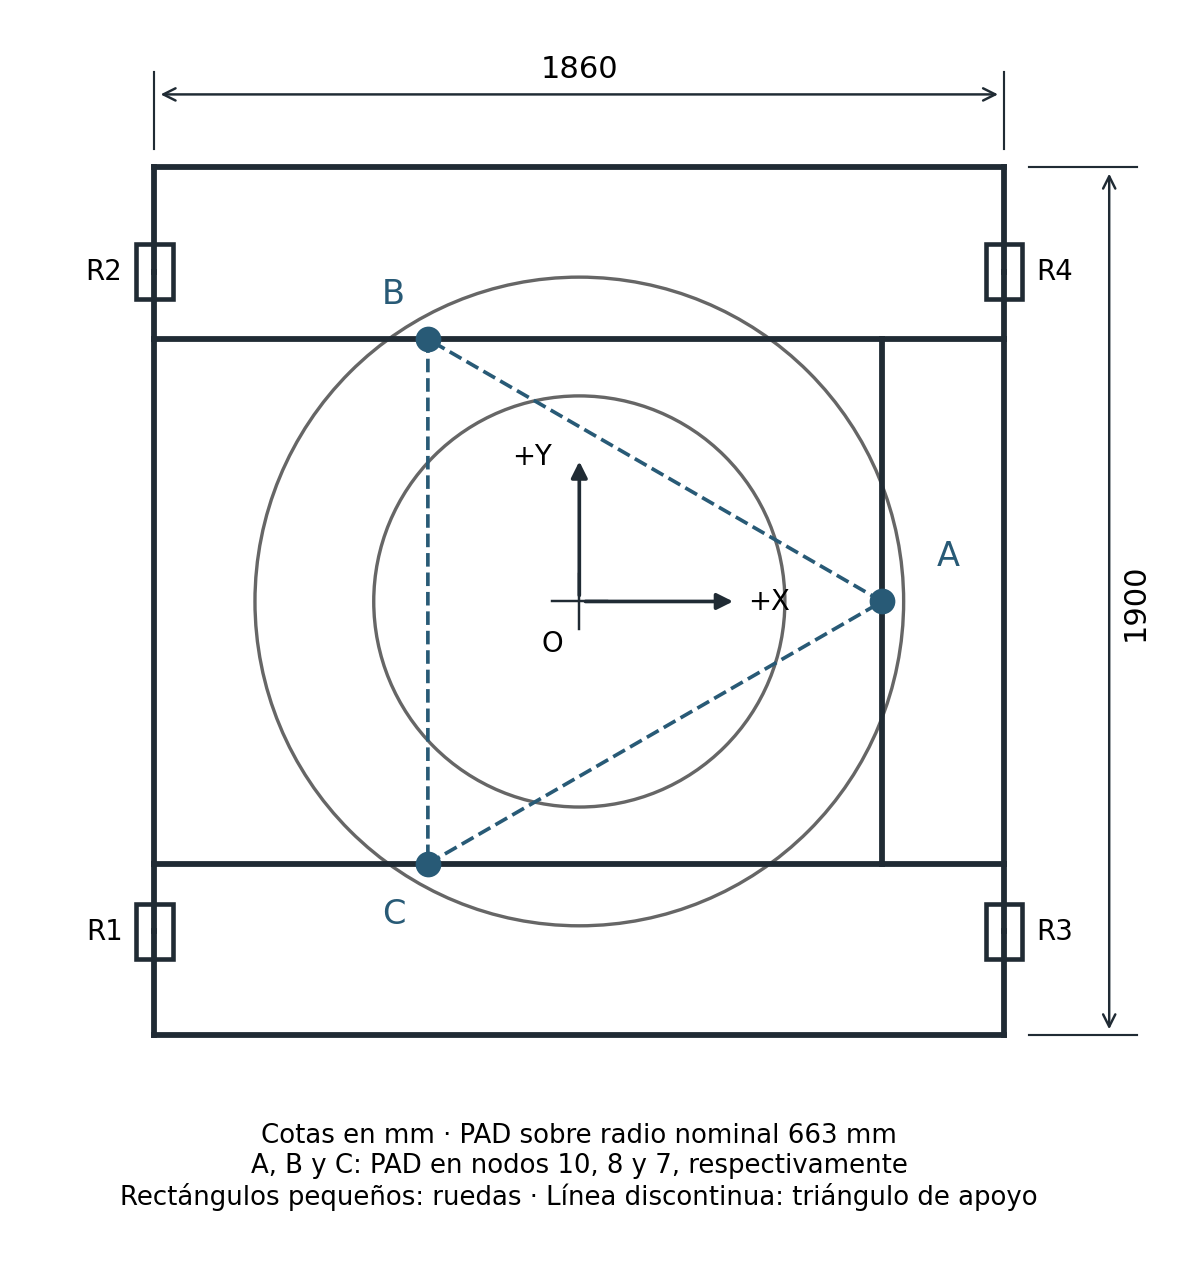
\includegraphics[width=0.92\textwidth]{images/planta_caso_manual}
\caption{Planta de cálculo reconstruida a partir de las coordenadas y la conectividad de la hoja exportada de SAP2000. El rodamiento está centrado; las barras se representan por sus líneas medias. Elaboración propia.}
\label{fig:planta_manual_revision}
\end{figure}

La Tabla~\ref{tab:coordenadas_manual_revision} recoge las coordenadas empleadas en el caso manual.

\begin{table}[htbp]
\centering\small\singlespacing
\caption{Posiciones utilizadas en el cálculo nominal}
\label{tab:coordenadas_manual_revision}
\begin{tabular}{lrrl}
\toprule
\textbf{Elemento} & \textbf{$X$ (mm)} & \textbf{$Y$ (mm)} & \textbf{Nodo SAP}\\
\midrule
Apoyo A & 663,00 & 0,00 & 10\\
Apoyo B & $-331,50$ & 574,18 & 8\\
Apoyo C & $-331,50$ & $-574,18$ & 7\\
Rueda 1 & $-930,00$ & $-722,00$ & 2\\
Rueda 2 & $-930,00$ & 722,00 & 5\\
Rueda 3 & 930,00 & $-722,00$ & 13\\
Rueda 4 & 930,00 & 722,00 & 16\\
\bottomrule
\end{tabular}
\par\smallskip\footnotesize
Fuente: tabla de coordenadas nodales de la exportación original de SAP2000 (Anexo~\ref{anx:programas}). La ordenada 574,18 mm conserva el redondeo de esa exportación; el valor geométrico nominal es aproximadamente 574,175 mm.
\end{table}

\subsubsection{Resolución del equilibrio del rodamiento}

Se aplica el equilibrio de fuerzas y momentos con las reacciones positivas hacia arriba \cite{shigley2015}. Para una resultante vertical que pasa por $(x_r,y_r)$, las ecuaciones son
\begin{equation}
\begin{bmatrix}
1&1&1\\
663&-331{,}5&-331{,}5\\
0&574{,}18&-574{,}18
\end{bmatrix}
\begin{bmatrix}R_A\\R_B\\R_C\end{bmatrix}
=
\begin{bmatrix}W_r\\W_r x_r\\W_r y_r\end{bmatrix}.
\label{eq:manual_matriz_pad}
\end{equation}
La primera fila se expresa en N; las dos restantes, en N\,mm. Para el caso centrado se reemplazan $x_r=y_r=0$ y $W_r=29844$ N:
\begin{align}
R_A+R_B+R_C &=29844,\\
663R_A-331{,}5R_B-331{,}5R_C&=0,\\
574{,}18R_B-574{,}18R_C&=0.
\end{align}
De la tercera ecuación se obtiene $R_B=R_C$. Al sustituir esta relación en la segunda, resulta $663R_A-663R_B=0$ y, por tanto, $R_A=R_B$. Finalmente,
\begin{equation}
\boxed{R_A=R_B=R_C=9948\ \mathrm{N}=9{,}948\ \mathrm{kN}.}
\label{eq:manual_reacciones_pad}
\end{equation}

La suma de las reacciones es 29844 N y sus momentos respecto de los dos ejes se anulan. Sobre el bastidor actúan las fuerzas opuestas, dirigidas hacia abajo. Estas fuerzas coinciden con los tres valores $F_3=-9948$ N registrados en la hoja de cargas nodales. Esa hoja contiene las cargas introducidas en SAP; no es un resultado de una simulación del contacto entre el rodamiento y los apoyos.

Para extender el cálculo a una resultante excéntrica, la resolución de la misma matriz da
\begin{align}
R_A&=\frac{W_r}{3}\left(1+\frac{2x_r}{663}\right),\\
R_B&=\frac{W_r-R_A}{2}+\frac{W_r y_r}{2(574{,}18)},\\
R_C&=\frac{W_r-R_A}{2}-\frac{W_r y_r}{2(574{,}18)}.
\label{eq:manual_pad_general}
\end{align}
Estas expresiones permiten evaluar otras posiciones de la resultante con las mismas coordenadas de apoyo, sin repetir su desarrollo algebraico.

\subsubsection{Contacto compresivo y presión media}

En una interfaz sin amarre vertical se exige reacción normal no negativa. Si $g_i$ representa la separación entre superficies, las condiciones ideales son
\begin{equation}
R_i\geq0,\qquad g_i\geq0,\qquad R_i g_i=0.
\label{eq:manual_contacto}
\end{equation}
Para el caso centrado se adopta la hipótesis de tres apoyos asentados, $g_A=g_B=g_C=0$. Las tres reacciones calculadas son positivas, de modo que la hipótesis es estáticamente admisible. Esta comprobación corresponde a apoyos puntuales ideales; no determina la distribución real de presión en un revestimiento deformable.

El área geométrica de cada liner, representado por un sector entre radios de 638 y 688 mm y ángulo de $24^\circ$, resulta
\begin{equation}
A=\frac{24\pi}{360}\left(688^2-638^2\right)
=13885{,}840\ \mathrm{mm^2}.
\label{eq:manual_area}
\end{equation}
Si toda esa área participa en el contacto, la presión media del caso nominal es
\begin{equation}
\boxed{p_m=\frac{9948}{13885{,}840}=0{,}7164\ \mathrm{MPa}.}
\label{eq:manual_presion}
\end{equation}
El resultado establece una demanda media de referencia. Para comprobar el liner se necesita el área efectiva y la resistencia admisible correspondiente a su material, temperatura y duración de la carga. Si la huella efectiva disminuye, la presión media aumenta.

La factibilidad se evalúa antes de aceptar una reacción máxima. Como comprobación del procedimiento, una resultante situada en $x_r=-400$ mm y $y_r=0$ produce
\[
R_A=-2055{,}620\ \mathrm{N},\qquad
R_B=R_C=15949{,}810\ \mathrm{N}.
\]
La reacción negativa indica que esa terna no puede sostener la carga con contactos exclusivamente compresivos y se rechaza esa solución. No se sustituye el valor negativo por cero, porque así se perdería el equilibrio de momentos. Este ejemplo es una prueba matemática fuera del triángulo de apoyo, no una posición de trabajo del rodamiento (Figura~\ref{fig:contacto_manual_revision}).

En el caso nominal, la resultante permanece dentro del triángulo y las tres reacciones son compresivas. La tolerancia propuesta de colocación de 5 mm requiere además revisar la cobertura del aro sobre cada apoyo. El triángulo de apoyo y la huella real del liner representan comprobaciones geométricas diferentes.

\begin{figure}[htbp]
\centering
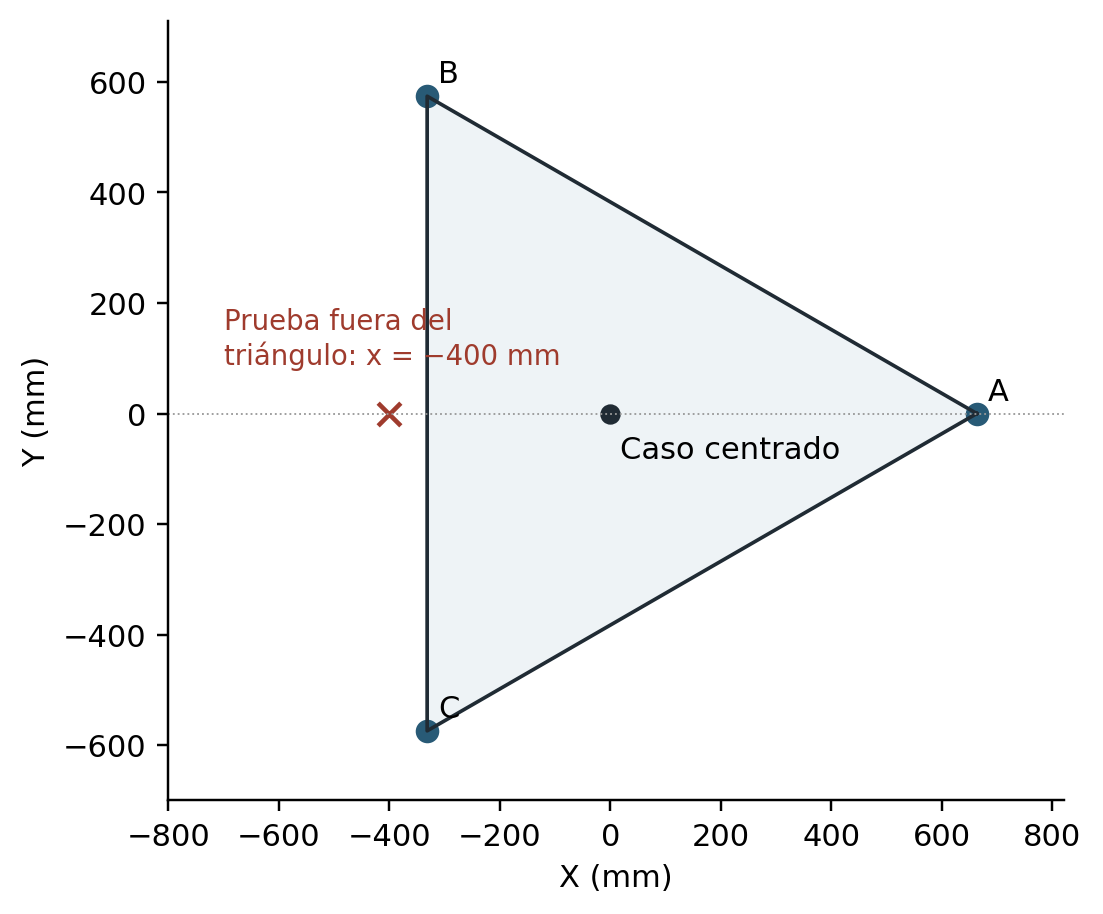
\includegraphics[width=0.84\textwidth]{images/factibilidad_pad}
\caption{Posición de la resultante del caso centrado y de la prueba matemática fuera del triángulo de apoyo. Elaboración propia a partir de las coordenadas del modelo.}
\label{fig:contacto_manual_revision}
\end{figure}

La Figura~\ref{fig:contacto_manual_revision} muestra ambas posiciones. El ejemplo exterior corresponde a una solución inadmisible porque exigiría tracción en un apoyo.

\subsubsection{Equilibrio del bastidor y reacciones en las ruedas}

La carga externa está centrada, pero la distribución de perfiles no es simétrica respecto de $X=0$: existe un miembro adicional en el lado del apoyo A. Para obtener el centro del peso propio se utilizan las longitudes y centroides de los 20 elementos de barra. Como todos tienen la misma sección y se adopta peso por unidad de longitud uniforme, el centro se calcula mediante
\begin{equation}
x_b=\frac{\sum_j L_j x_j}{\sum_j L_j},\qquad
y_b=\frac{\sum_j L_j y_j}{\sum_j L_j}.
\label{eq:manual_cg_perfiles}
\end{equation}
Con los valores de la tabla de conectividad de barras, se obtiene
\[
\sum_jL_j=12388{,}38\ \mathrm{mm},\quad
x_b=61{,}457808\ \mathrm{mm},\quad y_b\simeq0.
\]
El peso propio de barras se toma como una entrada del caso de referencia, $W_b=1648{,}74$ N. Su distribución se calcula a partir de la geometría, sin utilizar las reacciones individuales de SAP. El peso total y su primer momento respecto del plano $X=0$ son
\begin{align}
W_t&=29844+1648{,}74=31492{,}74\ \mathrm{N},\\
W_bx_b&=1648{,}74(61{,}457808)
=101327{,}946\ \mathrm{N\,mm}.
\label{eq:manual_peso_momento}
\end{align}

La geometría, las cargas y el campo vertical de la solución se consideran simétricos respecto de $Y=0$. En la idealización lineal de este caso, se conserva así la igualdad de las dos reacciones de cada lado: $R_1=R_2$ y $R_3=R_4$. Para evitar extender esta simplificación a otros escenarios, se limita a la carga vertical centrada y a los apoyos del modelo de referencia.

Al definir $R_-=R_1+R_2$ y $R_+=R_3+R_4$, el equilibrio exige
\begin{align}
R_-+R_+&=W_t,\\
930(R_+-R_-)&=W_bx_b.
\end{align}
Las reacciones individuales quedan
\begin{align}
R_1=R_2&=\frac{1}{4}\left(W_t-\frac{W_bx_b}{930}\right)
 =7845{,}9463\ \mathrm{N},\\
R_3=R_4&=\frac{1}{4}\left(W_t+\frac{W_bx_b}{930}\right)
 =7900{,}4237\ \mathrm{N}.
\label{eq:manual_ruedas}
\end{align}

La diferencia de carga entre ambos lados responde al centro del peso de los perfiles. El centro del rodamiento continúa en $(0,0)$. Tampoco debe confundirse este centro del bastidor analítico con el centro de gravedad del conjunto móvil, que incluye ruedas, mecanismos y otros accesorios. La Tabla~\ref{tab:manual_sap_revision} contrasta estas reacciones con las de la exportación de SAP2000.

\begin{table}[htbp]
\centering\small\singlespacing
\caption{Comparación de reacciones verticales del caso nominal}
\label{tab:manual_sap_revision}
\begin{tabular}{lrrr}
\toprule
\textbf{Nodo} & \textbf{Manual (N)} & \textbf{SAP (N)} & \textbf{Manual $-$ SAP (N)}\\
\midrule
2 & 7845,9463 & 7845,95 & $-0,0037$\\
5 & 7845,9463 & 7845,95 & $-0,0037$\\
13 & 7900,4237 & 7900,42 & 0,0037\\
16 & 7900,4237 & 7900,42 & 0,0037\\
\midrule
Total & 31492,7400 & 31492,74 & 0,0000\\
\bottomrule
\end{tabular}
\par\smallskip\footnotesize
Fuente: tabla de reacciones nodales de la exportación original de SAP2000, combinación nominal. El cálculo manual utiliza el peso propio total exportado y distribuye ese peso mediante la geometría de barras.
\end{table}

Las diferencias individuales son inferiores a 0,004 N, compatibles con la precisión de las tablas exportadas. El mayor error relativo es aproximadamente \SI{0.0000471}{\percent}. La comprobación confirma la suma y la distribución de reacciones del caso vertical centrado. No es una verificación independiente de la rigidez, del índice resistente ni de los contactos en situaciones de desnivel.

Las cuatro reacciones nominales son positivas. Este resultado es compatible con cuatro contactos cerrados en ese caso, pero los apoyos verticales del modelo SAP son bilaterales. La ausencia de levantamiento en otros escenarios requiere resolver las separaciones y reacciones de cada contacto; no se deduce de una sola combinación favorable.

\subsubsection{Cálculo manual de la flecha relativa a partir de SAP}

Se utiliza el travesaño comprendido entre los nodos 3 y 14, cuya luz es $L=1860$ mm. El nodo 7 está a $598{,}5$ mm del nodo 3. Para la combinación nominal, la exportación registra
\[
u_3=-0{,}117051\ \mathrm{mm},\quad
u_{14}=-0{,}117920\ \mathrm{mm},\quad
u_7=-1{,}353133\ \mathrm{mm}.
\]
La cuerda que une los extremos deformados tiene, en el nodo 7, el desplazamiento
\begin{align}
u_c&=u_3+\frac{598{,}5}{1860}(u_{14}-u_3)\\
&=-0{,}117330622\ \mathrm{mm}.
\end{align}
La flecha relativa absoluta es
\begin{equation}
\boxed{|\delta_{\mathrm{rel},7}|=|u_7-u_c|
=1{,}235802378\ \mathrm{mm}.}
\label{eq:manual_flecha}
\end{equation}
Para el criterio de proyecto propuesto,
\[
\frac{L}{800}=2{,}325\ \mathrm{mm},\qquad
\frac{|\delta_{\mathrm{rel},7}|}{L/800}=0{,}53153.
\]
El nodo evaluado queda por debajo de ese límite. La búsqueda del máximo a lo largo del miembro se realiza con las estaciones del modelo. El valor global $|U_3|$ no se reemplaza ni se confunde con la flecha relativa.

Este desarrollo muestra cómo se procesa un resultado de SAP. Una predicción manual independiente de desplazamiento requiere las inercias efectivas, las condiciones de unión y el modelo de cargas del elemento elegido, además del módulo elástico indicado en el apartado~\ref{sec:material-trazabilidad}. La interpolación de los desplazamientos exportados comprueba únicamente el posproceso.

\subsubsection{Extensión a los demás casos}

Las ecuaciones anteriores permiten extender el caso centrado a otras posiciones de la resultante y áreas de contacto. No se dispone de una hoja complementaria que reúna estas operaciones para los tres modelos de bastidor; el contraste se sustenta en el desarrollo explícito y las tablas originales, como se precisa en el apartado~\ref{sec:respaldo-complementario}. La comparación entre tres, cuatro y cinco apoyos emplea la misma carga externa total, con el reparto impuesto que se utilizó en los modelos disponibles:
\begin{equation}
P_{\mathrm{ap}}=\frac{W_r}{n}
\quad\Rightarrow\quad
9948;\ 7461;\ 5968{,}8\ \mathrm{N}
\quad\text{para } n=3,\ 4,\ 5.
\label{eq:manual_reparto_comparativo}
\end{equation}
Para tres apoyos no colineales, la carga centrada y el equilibrio justifican el reparto calculado. Para cuatro o cinco apoyos, el equilibrio vertical y los dos momentos no bastan para determinar todas las reacciones. Los valores iguales se conservan como cargas impuestas para comparar el bastidor; el contacto real requiere incorporar rigideces y compatibilidad de deformaciones.

Los desplazamientos y los índices resistentes se mantienen como resultados de las corridas originales. Modificar una masa en un cálculo analítico no actualiza esos resultados ni sustituye la solución del modelo estructural.

\section{Dimensionamiento analítico del sistema de aspersión}
\label{sec:man-asp-base}

El sistema de aspersión debe suministrar líquido a las superficies exteriores
y al agujero del rodamiento mientras la pieza permanece inmóvil sobre sus
tres apoyos. El distribuidor gira alrededor del eje vertical de la pieza y
alimenta dos ramales exteriores, un ramal interior y dos grupos superiores.
El dimensionamiento determina cuántas boquillas se requieren, cuánto
líquido debe circular, qué presión debe proporcionar la bomba y qué potencia
demanda el bombeo. La cobertura geométrica se evalúa por separado, porque
disponer de presión y caudal no demuestra por sí solo la remoción de grasa.

Se aplican la conservación de masa, el balance de energía de Bernoulli,
las pérdidas de Darcy--Weisbach y el balance de cantidad de movimiento.
Estas relaciones se desarrollan a continuación con los datos, las
sustituciones numéricas y la interpretación de cada resultado.

\subsection{Datos de diseño y supuestos de cálculo}
\label{sec:man-asp-datos}

El rodamiento de referencia es el SKF 241/900 ECAK30/W33. Sus diámetros
exterior e interior son 1420 y 900 mm, y su ancho axial es 515 mm
\cite{skf241}. En posición de lavado, el eje del rodamiento es vertical.
Las cotas $z$ de este desarrollo se miden desde el piso de la cabina; por
consiguiente, no se confunden con la distancia medida desde el centro de
la pieza. Se adoptan $z_{inf}=890$ mm y $z_{sup}=1405$ mm para sus caras. La
Tabla~\ref{tab:man-asp-base} reúne las condiciones geométricas y operativas del caso.

\begin{table}[htbp]
\centering\small
\caption{Condiciones geométricas y operativas del caso base.}
\label{tab:man-asp-base}
\begin{tabularx}{\linewidth}{@{}>{\raggedright\arraybackslash}X l >{\raggedright\arraybackslash}p{4.1cm}@{}}
\toprule Parámetro & Valor & Condición\\\midrule
Diámetro exterior $D$ & 1420 mm & Dato del rodamiento.\\
Diámetro interior menor $d$ & 900 mm & Agujero cónico 1:30.\\
Ancho axial $B$ & 515 mm & Dato del rodamiento.\\
Temperatura nominal $T$ & 62 $^\circ$C & Condición de diseño adoptada.\\
Presión mínima de boquilla $p_n$ & 4 bar & Presión manométrica propuesta.\\
Distancia lateral $s_e$ & 125,85 mm & Separación geométrica adoptada.\\
Distancia interior $s_i$ & 143,30 mm & Separación geométrica adoptada.\\
Distancia superior $s_s$ & 184,85 mm & Separación geométrica adoptada.\\
Ángulo de abanico $\theta$ & 50$^\circ$ & Ángulo de cálculo adoptado.\\
Solape mínimo objetivo $\phi$ & 25\,\% & Criterio geométrico propuesto.\\
\bottomrule
\end{tabularx}
\end{table}

Se supone régimen permanente, líquido incompresible y tuberías llenas.
El detergente diluido se aproxima inicialmente mediante las propiedades
del agua a 62 $^\circ$C. Esta simplificación permite predimensionar la red;
deberá revisarse al conocer la formulación y concentración del producto.
Las propiedades se obtuvieron de la biblioteca CoolProp, que implementa
las formulaciones de referencia para el agua \cite{bell2014}:
\begin{equation}
 \rho=982{,}120\ \mathrm{kg/m^3},\qquad
 \mu=4{,}52269\times10^{-4}\ \mathrm{Pa\,s},\qquad
 p_v=21866{,}997\ \mathrm{Pa}.
 \label{eq:man-asp-props}
\end{equation}
La viscosidad cinemática se obtiene dividiendo la viscosidad dinámica por
la densidad:
\begin{equation}
 \nu=\frac{\mu}{\rho}
 =\frac{4{,}52269\times10^{-4}\ \mathrm{kg/(m\,s)}}
 {982{,}120\ \mathrm{kg/m^3}}
 =4{,}60503\times10^{-7}\ \mathrm{m^2/s}.
 \label{eq:man-asp-nu}
\end{equation}
Se utiliza $g=9{,}81$ m/s$^2$. En la hidráulica, $Q$ representa el caudal
de una tubería y $q$ el caudal de una boquilla. Los cálculos de pérdidas
se efectúan en metros, segundos y pascales; en la geometría de huellas
se mantienen milímetros. Un bar equivale a $10^5$ Pa y un L/min a
$1/60000$ m$^3$/s.

\subsection{Caudal y velocidad de una boquilla}
\label{sec:man-asp-boquilla}

Se toma como referencia hidráulica una boquilla de abanico plano H3/8U-5020,
cuya ficha indica 2 gal/min estadounidenses a 40 psi y un diámetro equivalente
de 0,109 pulgadas \cite{manSpray}. Se emplea su capacidad para el cálculo,
sin considerar cerrado el material comercial de la boquilla ni su
compatibilidad con la solución de limpieza.

\subsubsection{Conversión del punto nominal}
El caudal y la presión de catálogo se convierten antes de aplicar las ecuaciones:
\begin{align}
 q_r&=2\ \frac{\mathrm{gal}}{\mathrm{min}}
 \left(3{,}785411784\ \frac{\mathrm{L}}{\mathrm{gal}}\right)
 =7{,}57082\ \mathrm{L/min},\label{eq:man-asp-qr}\\
 p_r&=40\ \mathrm{psi}\left(6894{,}757\ \frac{\mathrm{Pa}}{\mathrm{psi}}\right)
 =275790{,}28\ \mathrm{Pa}=2{,}75790\ \mathrm{bar}.
 \label{eq:man-asp-pr}
\end{align}

\subsubsection{Caudal a la presión de diseño}
Para el mismo orificio y propiedades aproximadamente constantes,
$q$ varía con la raíz cuadrada de la presión diferencial. Así,
\begin{equation}
 q=q_r\sqrt{\frac{p_n}{p_r}}
 =7{,}57082\sqrt{\frac{4{,}00000}{2{,}75790}}
 =\boxed{9{,}11767\ \mathrm{L/min}}.
 \label{eq:man-asp-q}
\end{equation}
La presión de la Ecuación~\eqref{eq:man-asp-q} es la diferencia entre la
entrada de la boquilla y la cabina, considerada a presión atmosférica.
No es la presión absoluta del líquido. La misma relación puede escribirse
como $q=K_q\sqrt{p_n}$, con
\begin{equation}
 K_q=\frac{7{,}57082}{\sqrt{2{,}75790}}
 =4{,}55883\ \frac{\mathrm{L}}{\mathrm{min}\sqrt{\mathrm{bar}}}.
 \label{eq:man-asp-kq}
\end{equation}
Este coeficiente se utiliza después para actualizar el caudal de cada
boquilla cuando su presión difiere ligeramente de 4 bar. Se conserva el
coeficiente nominal de catálogo; la variación por temperatura y detergente
debe comprobarse con el fabricante.

\subsubsection{Velocidad y escala de fuerza del chorro}
Se adopta un coeficiente de velocidad $C_v=0{,}95$ como hipótesis. La
velocidad característica estimada es
\begin{equation}
 v_j=C_v\sqrt{\frac{2p_n}{\rho}}
 =0{,}95\sqrt{\frac{2(400000)}{982{,}120}}
 =\boxed{27{,}114\ \mathrm{m/s}}.
 \label{eq:man-asp-vj}
\end{equation}
Primero se convierte el caudal a SI:
\begin{equation}
 q=\frac{9{,}11767}{60000}=1{,}51961\times10^{-4}\ \mathrm{m^3/s}.
\end{equation}
El flujo de cantidad de movimiento proporciona una escala de fuerza:
\begin{equation}
 F\simeq\rho qv_j
 =(982{,}120)(1{,}51961\times10^{-4})(27{,}114)
 =\boxed{4{,}047\ \mathrm{N}}.
 \label{eq:man-asp-f}
\end{equation}
Esta fuerza corresponde a una representación equivalente del chorro. No
es una medición de impacto sobre la grasa ni un valor de esfuerzo cortante
de pared; ambos dependen de la distribución real del abanico y de la distancia.

Como comprobación dimensional del orificio,
$d_{eq}=0{,}109(25{,}4)=2{,}7686$ mm y
$A_{eq}=\pi(0{,}0027686)^2/4=6{,}02019\times10^{-6}$ m$^2$.
El coeficiente de descarga implícito resulta
\begin{equation}
 C_d=\frac{q}{A_{eq}\sqrt{2p_n/\rho}}
 =\frac{1{,}51961\times10^{-4}}
 {(6{,}02019\times10^{-6})(28{,}5406)}
 \simeq0{,}884.
 \label{eq:man-asp-cd}
\end{equation}
El área es equivalente: no representa necesariamente un orificio circular
real ni permite reemplazar el abanico por un chorro cilíndrico en una
simulación sin justificar esa idealización.

\subsection{Número de boquillas y cobertura nominal}
\label{sec:man-asp-cobertura}

Una boquilla de abanico plano situada a distancia $s$, con incidencia normal,
produce una anchura geométrica
\begin{equation}
 b=2s\tan(\theta/2).
 \label{eq:man-asp-b}
\end{equation}
La ecuación se obtiene de los dos triángulos rectángulos formados por el eje
del chorro y sus rayos extremos. Describe la envolvente ideal del abanico,
no una distribución uniforme de caudal sobre toda la huella.

Si dos huellas de ancho $b$ deben superponerse una fracción $\phi$, la
separación máxima entre centros es $a_{max}=b(1-\phi)$. Con $N$ boquillas,
la longitud cubierta es $b+(N-1)a_{max}$. Para cubrir una longitud $L$ se exige
\begin{equation}
 b+(N-1)b(1-\phi)\geq L
 \quad\Longrightarrow\quad
 N\geq1+\frac{L-b}{b(1-\phi)}.
 \label{eq:man-asp-n}
\end{equation}
Se redondea hacia arriba porque la cantidad de boquillas debe ser entera,
con un mínimo de una.

\subsubsection{Ramal interior}
La longitud objetivo es el ancho axial del rodamiento, $L=515$ mm:
\begin{align}
 b_i&=2(143{,}30)\tan25^\circ=133{,}644\ \mathrm{mm},\\
 N_i&\geq1+\frac{515-133{,}644}{133{,}644(1-0{,}25)}
 =4{,}805\quad\Longrightarrow\quad\boxed{N_i=5}.
\end{align}
Una vez fijado $N_i$, se distribuyen sus centros uniformemente:
\begin{align}
 a_i&=\frac{515-133{,}644}{5-1}=95{,}339\ \mathrm{mm},\\
 \phi_i&=1-\frac{95{,}339}{133{,}644}=0{,}2866.
\end{align}
El solape nominal es 28,66\,\%, superior al 25\,\% propuesto.
La primera boquilla queda a $890+b_i/2=956{,}822$ mm y las siguientes
a esa cota más múltiplos de $a_i$. Así se obtienen, redondeando a décimas,
$z=956{,}8;1052{,}2;1147{,}5;1242{,}8;1338{,}2$ mm.

\subsubsection{Grupos superiores}
La anchura radial de la cara anular es
$L_s=(1420-900)/2=260$ mm. Por cada lado del distribuidor:
\begin{align}
 b_s&=2(184{,}85)\tan25^\circ=172{,}394\ \mathrm{mm},\\
 N_s&\geq1+\frac{260-172{,}394}{172{,}394(0{,}75)}
 =1{,}678\quad\Longrightarrow\quad\boxed{N_s=2},\\
 a_s&=\frac{260-172{,}394}{2-1}=87{,}606\ \mathrm{mm}.
\end{align}
Sus radios nominales son $450+b_s/2=536{,}197$ mm y
$536{,}197+87{,}606=623{,}803$ mm. Se requieren cuatro boquillas
superiores en total. El solape radial nominal es 49,18\,\%.
La cobertura sobre la proyección anular no demuestra el alcance de las
superficies internas entre aros, rodillos y jaula.

\subsubsection{Ramales exteriores}
Se obtiene $b_e=2(125{,}85)\tan25^\circ=117{,}370$ mm.
El caso base dispone cuatro boquillas de eje radial por ramal, con centros
entre 1100 mm y $1405-b_e/2=1346{,}315$ mm. Su separación es
\begin{equation}
 a_e=\frac{1346{,}315-1100}{4-1}=82{,}105\ \mathrm{mm},\qquad
 \phi_e=1-\frac{82{,}105}{117{,}370}=0{,}3005.
\end{equation}
Estas cuatro boquillas cubren nominalmente desde
$1100-117{,}370/2=1041{,}315$ mm hasta 1405 mm. El solape de
30,05\,\% se refiere únicamente a ellas. Para intentar alcanzar la zona
inferior se propone una quinta boquilla inclinada en cada ramal.

\subsubsection{Comprobación de la boquilla inclinada}
Su centro está a $z_n=1070$ mm y su eje apunta hacia $z_t=950$ mm.
La inclinación descendente es
\begin{equation}
 \alpha=\arctan\left(\frac{1070-950}{125{,}85}\right)=43{,}637^\circ.
\end{equation}
En un plano radial vertical, cada rayo recorre horizontalmente $s_e$ hasta
la generatriz del rodamiento. Sus descensos son $s_e\tan(\alpha\pm25^\circ)$;
por tanto, los bordes no son simétricos respecto del punto de impacto del eje:
\begin{align}
 z_{min}&=1070-125{,}85\tan(43{,}637^\circ+25^\circ)
 =748{,}259\ \mathrm{mm},\\
 z_{max}&=1070-125{,}85\tan(43{,}637^\circ-25^\circ)
 =1027{,}557\ \mathrm{mm}.
 \label{eq:man-asp-inclinada}
\end{align}
La intersección de esta huella ideal con la superficie exterior existente
comienza a 890 mm. Entre su borde superior y la huella radial siguiente queda
\begin{equation}
 \Delta z_{sin\ cobertura}=1041{,}315-1027{,}557
 =\boxed{13{,}759\ \mathrm{mm}}.
 \label{eq:man-asp-hueco}
\end{equation}
En consecuencia, la distribución lateral propuesta no garantiza cobertura
axial completa en esta posición nominal. Debe ajustarse la orientación o la
ubicación de la boquilla y comprobarse el barrido con oscilación y las sombras
del soporte. El cálculo hidráulico posterior corresponde a esta configuración
base de 19 boquillas, cuya distribución detalla la
Tabla~\ref{tab:man-asp-cantidad}; no implica que el problema de cobertura esté resuelto.

\begin{table}[htbp]
\centering\small
\caption{Cantidad de boquillas del caso base hidráulico.}
\label{tab:man-asp-cantidad}
\begin{tabularx}{\linewidth}{@{}Xrr@{}}
\toprule Grupo & Distribución & Total\\\midrule
Ramales exteriores & $2(4+1)$ & 10\\
Ramal interior & $1(5)$ & 5\\
Grupos superiores & $2(2)$ & 4\\\midrule
Total simultáneo & & 19\\\bottomrule
\end{tabularx}
\end{table}

\subsection{Primera estimación del caudal total}
\label{sec:man-asp-qtotal}
Si todas las boquillas reciben exactamente 4 bar, el caudal es
\begin{equation}
 Q_0=Nq=19(9{,}11767)
 =173{,}236\ \mathrm{L/min}
 =2{,}88726\times10^{-3}\ \mathrm{m^3/s}.
 \label{eq:man-asp-q0}
\end{equation}
Esta es una primera estimación por continuidad, no un caudal asignado a
cada tubo del distribuidor. Cada tramo transporta la suma de las boquillas
que tiene aguas abajo. La diferencia de elevación y las pérdidas generan
presiones ligeramente distintas; la sección siguiente determina esa
corrección y el caudal que se empleará en la alimentación principal.
\subsection{Modelo hidráulico y cálculo de la distribución}
\label{sec:man-asp-red}

Se identifica como $C$ la salida de alimentación central, situada a
$z_C=1{,}770$ m. Desde ella parten dos recorridos exteriores simétricos
y un recorrido interior. En cada lado exterior, $S1$ y $S2$ son las tomas
superiores; $E0$ es el inicio del tubo descendente y $E1$ a $E5$ son sus
tomas. En el ramal interior, $I0$ es la entrada y $I1$ a $I5$ son las
tomas ordenadas de arriba hacia abajo. Los puntos de la
Figura~\ref{fig:man-asp-esquema} son estaciones de cálculo, no un plano
de montaje.

\begin{figure}[htbp]
\centering
\begin{tikzpicture}[>=Stealth, every node/.style={font=\small},
 box/.style={draw,rounded corners=2pt,align=center,minimum height=10mm,text width=24mm},
 flow/.style={->,thick}]
\node[box] (tan) at (0,0) {Depósito\\abierto};
\node[box] (bom) at (3.3,0) {Bomba};
\node[box] (fil) at (6.6,0) {Filtro};
\node[box] (uni) at (9.9,0) {Unión\\rotativa};
\draw[flow] (tan)--node[above,font=\scriptsize]{DN50}(bom);
\draw[flow] (bom)--node[above,font=\scriptsize]{DN40}(fil);
\draw[flow] (fil)--node[above,font=\scriptsize]{DN40}(uni);
\node[box] (c) at (9.9,-1.8) {$C$\\Distribución};
\draw[flow] (uni)--node[right,font=\scriptsize]{DN40}(c);
\node[box,text width=34mm] (a) at (0,-3.6) {Lado exterior 1\\$S1,S2,E1\ldots E5$\\7 boquillas};
\node[box,text width=34mm] (b) at (4.9,-3.6) {Lado exterior 2\\Simétrico al lado 1\\7 boquillas};
\node[box,text width=34mm] (i) at (9.9,-3.6) {Ramal interior\\$I1\ldots I5$\\5 boquillas};
\draw[flow] (c.west)--(0,-1.8)--(a.north);
\draw[flow] (4.9,-1.8)--(b.north);
\draw[flow] (c)--(i);
\node[align=center,text width=12cm] at (4.9,-5) {Después de la aplicación, el líquido retorna al depósito.\\El dimensionamiento del retorno y del tanque se evalúa por separado.};
\end{tikzpicture}
\caption{Esquema funcional del circuito y de los grupos simultáneos. Elaboración propia; sin escala.}
\label{fig:man-asp-esquema}
\end{figure}

\subsubsection{Geometría hidráulica adoptada}
Se consideran diámetros exteriores de 33,4; 48,3 y 60,3 mm, con espesor
de 2,77 mm. El diámetro que interviene en la velocidad es el interior:
\begin{equation}
 D_{25}=33{,}4-2(2{,}77)=27{,}86\ \mathrm{mm},\quad
 D_{40}=42{,}76\ \mathrm{mm},\quad D_{50}=54{,}76\ \mathrm{mm}.
\end{equation}
Estas dimensiones se adoptan para el predimensionamiento y deben cotejarse
con la tubería suministrada. Se supone rugosidad $\varepsilon=0{,}045$ mm.

\subsubsection{Ecuaciones por tramo}
Para cada tubo se calculan la velocidad, Reynolds y factor de Darcy:
\begin{align}
 v&=\frac{4Q}{\pi D_i^2},\qquad Re=\frac{\rho vD_i}{\mu},
 \label{eq:man-asp-vre}\\
 f&=\frac{0{,}25}{\left[\log_{10}\left(
 \frac{\varepsilon}{3{,}7D_i}+\frac{5{,}74}{Re^{0{,}9}}\right)\right]^2}.
 \label{eq:man-asp-sj}
\end{align}
La Ecuación~\eqref{eq:man-asp-sj} es la aproximación de Swamee--Jain para
el régimen turbulento \cite{manSwamee}. Las pérdidas del tramo son
\begin{equation}
 h_L=h_f+h_m
 =\left(f\frac{L}{D_i}+\sum K_m\right)\frac{v^2}{2g}.
 \label{eq:man-asp-hl}
\end{equation}
Los coeficientes $K_m$ son adimensionales y se refieren a la velocidad del
tramo donde se colocan. No deben confundirse con el coeficiente de boquilla
$K_q$. Para el caso base se adoptan factores $f_T$ de 0,023; 0,020 y 0,019
para DN25, DN40 y DN50; se representan un paso de derivación por $20f_T$,
una salida de derivación por $60f_T$ y un codo por $30f_T$.
Son coeficientes de predimensionamiento, sujetos a confirmación con los
accesorios reales. Por ejemplo, la entrada a un lado exterior toma
$60(0{,}019)=1{,}14$, y la entrada interior,
$(60+30)(0{,}023)=2{,}07$.

\subsubsection{Relación entre presión, caudal y elevación}
En un tramo sin bomba, Bernoulli proporciona
\begin{equation}
 \frac{p_j}{\rho g}+z_j+\frac{v_j^2}{2g}
 =\frac{p_i}{\rho g}+z_i+\frac{v_i^2}{2g}-h_{L,ij}.
 \label{eq:man-asp-bernoulli-ramal}
\end{equation}
Para la primera aproximación de los colectores se desprecia la diferencia
de cargas cinéticas entre sus estaciones. Así,
\begin{equation}
 p_j\simeq p_i-\rho g\left[h_{L,ij}+(z_j-z_i)\right],\qquad
 q_j=K_q\sqrt{p_j},
 \label{eq:man-asp-recursion}
\end{equation}
con $p_j$ en bar únicamente en la segunda expresión, por las unidades
elegidas para $K_q$. La primera expresión emplea pascales.
La menor elevación incrementa la presión; la pérdida de carga la reduce.
Las tomas superiores se representan a 1,740 m, en el colector. El descenso
dentro del cuerpo y de las conexiones de cada boquilla no se modela.
Las diferencias cinéticas y estas conexiones se deben incluir al cerrar
la red; por ello se presenta un predimensionamiento, no una predicción
exacta de la instalación.

\subsubsection{Procedimiento de solución por aproximaciones sucesivas}
Se inicia con $q_j=9{,}11767$ L/min y $p_C=4$ bar. Se suman los caudales
aguas abajo de cada tramo, se calculan sus pérdidas y se obtienen las
presiones con la Ecuación~\eqref{eq:man-asp-recursion}. Después se actualiza
cada caudal con su presión y se ajusta la presión central mediante
\begin{equation}
 p_C^{(k+1)}=p_C^{(k)}+\left(4-p_{min}^{(k)}\right)
 \quad[\mathrm{bar}].
 \label{eq:man-asp-iteracion}
\end{equation}
Así se busca que la toma más desfavorable tenga 4 bar. Es una resolución
de ecuaciones de continuidad y energía; las sucesivas aproximaciones se
exponen para que el cálculo pueda comprobarse con una calculadora: la
Tabla~\ref{tab:man-asp-iteraciones} registra las aproximaciones y la
Tabla~\ref{tab:man-asp-tramos}, los tramos del estado convergido.

\begin{table}[htbp]
\centering\small
\caption{Aproximaciones sucesivas para determinar la presión central.}
\label{tab:man-asp-iteraciones}
\begin{tabular}{@{}rrrr@{}}
\toprule
Iteración & $p_C$ (bar) & $p_{\min}$ (bar) & $Q$ actualizado (L/min)\\\midrule
0 & 4{,}000000 & 4{,}001211 & 174{,}019197\\
1 & 3{,}998789 & 3{,}999984 & 173{,}991281\\
2 & 3{,}998805 & 4{,}000001 & 173{,}991697\\
3 & 3{,}998805 & 4{,}000000 & 173{,}991684\\
\bottomrule
\end{tabular}
\end{table}
En las dos últimas filas la diferencia de caudal total es menor que
0,001 L/min. Los dígitos adicionales permiten revisar el cierre aritmético;
no representan la precisión física de las hipótesis.

\begin{table}[htbp]
\centering\small
\caption{Datos por tramo y pérdidas del estado convergido.}
\label{tab:man-asp-tramos}
\begin{tabular}{@{}lrrrrrr@{}}
\toprule
Tramo & DN & $L$ (m) & $\sum K_m$ & $Q$ (L/min) & $h_L$ (m) & $z_f$ (m)\\\midrule
C--S1 & 50 & 0{,}5360 & 1{,}140 & 64{,}113 & 0{,}01436 & 1{,}7400\\
S1--S2 & 50 & 0{,}0880 & 0{,}380 & 54{,}995 & 0{,}00323 & 1{,}7400\\
S2--E0 & 50 & 0{,}2760 & 0{,}950 & 45{,}877 & 0{,}00577 & 1{,}7400\\
E0--E1 & 40 & 0{,}3940 & 0{,}400 & 45{,}877 & 0{,}00902 & 1{,}3460\\
E1--E2 & 40 & 0{,}0820 & 0{,}400 & 36{,}718 & 0{,}00415 & 1{,}2640\\
E2--E3 & 40 & 0{,}0820 & 0{,}400 & 27{,}550 & 0{,}00235 & 1{,}1820\\
E3--E4 & 40 & 0{,}0820 & 0{,}400 & 18{,}374 & 0{,}00105 & 1{,}1000\\
E4--E5 & 40 & 0{,}0300 & 0{,}400 & 9{,}188 & 0{,}00025 & 1{,}0700\\
C--I0 & 25 & 0{,}2800 & 2{,}070 & 45{,}766 & 0{,}18508 & 1{,}7400\\
I0--I1 & 25 & 0{,}4018 & 0{,}460 & 45{,}766 & 0{,}06526 & 1{,}3382\\
I1--I2 & 25 & 0{,}0954 & 0{,}460 & 36{,}630 & 0{,}02795 & 1{,}2428\\
I2--I3 & 25 & 0{,}0953 & 0{,}460 & 27{,}486 & 0{,}01581 & 1{,}1475\\
I3--I4 & 25 & 0{,}0953 & 0{,}460 & 18{,}334 & 0{,}00710 & 1{,}0522\\
I4--I5 & 25 & 0{,}0954 & 0{,}460 & 9{,}172 & 0{,}00181 & 0{,}9568\\
\bottomrule
\end{tabular}
\par\smallskip\footnotesize
Se muestra un lado exterior; el segundo es simétrico. $z_f$ es la elevación
final del tramo. Los caudales y pérdidas son resultados; $L$, DN y
$\sum K_m$ son entradas del modelo.
\end{table}

\subsubsection{Ejemplo completo: primer tramo del lado exterior}
El tramo $C$--$S1$ alimenta siete boquillas. En el estado convergido conduce
$Q=64{,}11274$ L/min $=1{,}06855\times10^{-3}$ m$^3$/s. Se tiene
$D_i=0{,}05476$ m, $L=0{,}536$ m y $\sum K_m=1{,}14$. Entonces:
\begin{align}
 v&=\frac{4(1{,}06855\times10^{-3})}{\pi(0{,}05476)^2}
 =0{,}45371\ \mathrm{m/s},\\
 Re&=\frac{982{,}120(0{,}45371)(0{,}05476)}{4{,}52269\times10^{-4}}
 =5{,}3952\times10^4,\\
 f&=\frac{0{,}25}{\left[\log_{10}\left(
 \frac{0{,}000045}{3{,}7(0{,}05476)}+
 \frac{5{,}74}{(53952)^{0{,}9}}\right)\right]^2}=0{,}023396,\\
 h_{L,C-S1}&=\left(0{,}023396\frac{0{,}536}{0{,}05476}+1{,}14\right)
 \frac{0{,}45371^2}{2(9{,}81)}=0{,}014363\ \mathrm{m}.
\end{align}
El segundo tramo, $S1$--$S2$, conduce el caudal restante después de la
primera boquilla y pierde 0,003230 m. Como $S2$ es la toma desfavorable,
la presión central se puede verificar directamente:
\begin{align}
 p_C&=p_{S2}+\rho g\left[h_{L,C-S1}+h_{L,S1-S2}+z_{S2}-z_C\right]\notag\\
 &=400000+982{,}120(9{,}81)
 \left(0{,}014363+0{,}003230+1{,}740-1{,}770\right)\notag\\
 &=\boxed{399880{,}47\ \mathrm{Pa}=3{,}99880\ \mathrm{bar}}.
 \label{eq:man-asp-pc}
\end{align}
El resultado es ligeramente inferior a 4 bar porque el descenso de 30 mm
aporta más presión hidrostática que la perdida en esos dos tramos. La
Tabla~\ref{tab:man-asp-boquillas} reúne la presión y el caudal de cada toma.

\begin{table}[htbp]
\centering\small
\caption{Presión y caudal calculados en las tomas de boquilla.}
\label{tab:man-asp-boquillas}
\begin{tabular}{@{}lrrrr@{}}
\toprule
Punto & Cantidad & $z$ (m) & $p_g$ (bar) & $q$ (L/min)\\\midrule
S1 & 2 & 1{,}7400 & 4{,}00031 & 9{,}11802\\
S2 & 2 & 1{,}7400 & 4{,}00000 & 9{,}11767\\
E1 & 2 & 1{,}3460 & 4{,}03653 & 9{,}15921\\
E2 & 2 & 1{,}2640 & 4{,}04404 & 9{,}16772\\
E3 & 2 & 1{,}1820 & 4{,}05171 & 9{,}17641\\
E4 & 2 & 1{,}1000 & 4{,}05951 & 9{,}18524\\
E5 & 2 & 1{,}0700 & 4{,}06238 & 9{,}18848\\
I1 & 1 & 1{,}3382 & 4{,}01629 & 9{,}13621\\
I2 & 1 & 1{,}2428 & 4{,}02279 & 9{,}14360\\
I3 & 1 & 1{,}1475 & 4{,}03044 & 9{,}15230\\
I4 & 1 & 1{,}0522 & 4{,}03894 & 9{,}16194\\
I5 & 1 & 0{,}9568 & 4{,}04796 & 9{,}17216\\
\bottomrule
\end{tabular}
\par\smallskip\footnotesize
La cantidad 2 corresponde a puntos equivalentes en los dos lados exteriores.
Los puntos $I1$--$I5$ pertenecen a un único ramal interior.
\end{table}

La suma de un lado exterior es 64,11274 L/min y la del ramal interior
45,76621 L/min. Por continuidad, el caudal final es
\begin{equation}
 Q=2(64{,}11274)+45{,}76621
 =\boxed{173{,}99168\ \mathrm{L/min}}
 =\boxed{2{,}89986\times10^{-3}\ \mathrm{m^3/s}}.
 \label{eq:man-asp-qfinal}
\end{equation}
La variación respecto de $Q_0=173{,}23564$ L/min es 0,44\,\%.
Las boquillas inferiores entregan algo más de líquido al recibir más
presión. La dispersión extrema de caudal predicha es
\begin{equation}
 \delta_q=100\left(\sqrt{\frac{4{,}06238}{4{,}00000}}-1\right)
 =0{,}777\ \mathord{\text{\%}}.
\end{equation}
Esta dispersión se refiere al caudal de las boquillas del modelo; no es
un indicador de uniformidad de limpieza sobre la pieza.

\subsection{Diámetro de alimentación y pérdidas de la línea principal}
\label{sec:man-asp-alimentacion}

Se adopta como criterio de predimensionamiento una velocidad de 1,5 a
3 m/s en la alimentación a presión. No se aplica ese intervalo como
restricción universal a todos los colectores. Para DN40,
\begin{equation}
 v_{40}=\frac{4(2{,}89986\times10^{-3})}{\pi(0{,}04276)^2}
 =\boxed{2{,}01935\ \mathrm{m/s}}.
 \label{eq:man-asp-v40}
\end{equation}
El Reynolds y el factor de Darcy son
\begin{align}
 Re_{40}&=\frac{982{,}120(2{,}01935)(0{,}04276)}{4{,}52269\times10^{-4}}
 =1{,}87507\times10^5,\\
 f_{40}&=\frac{0{,}25}{\left[\log_{10}\left(
 \frac{0{,}000045}{3{,}7(0{,}04276)}+
 \frac{5{,}74}{(187507)^{0{,}9}}\right)\right]^2}=0{,}021478.
\end{align}

\subsubsection{Línea estacionaria}
Se adopta una longitud de 14 m, seis codos, una válvula de retención y
una válvula de bola. La longitud y los accesorios son hipótesis de trazado.
Con $K_{codo}=0{,}60$, $K_{ret}=2{,}00$ y $K_{bola}=0{,}06$,
\begin{equation}
 \sum K_{est}=6(0{,}60)+2{,}00+0{,}06=5{,}66.
\end{equation}
La fricción distribuida y las pérdidas locales se calculan por separado:
\begin{align}
 h_{f,est}&=0{,}021478\frac{14}{0{,}04276}
 \frac{2{,}01935^2}{2(9{,}81)}=1{,}46154\ \mathrm{m},\\
 h_{m,est}&=5{,}66\frac{2{,}01935^2}{2(9{,}81)}=1{,}17636\ \mathrm{m},\\
 h_{L,est}&=1{,}46154+1{,}17636=\boxed{2{,}63790\ \mathrm{m}}.
 \label{eq:man-asp-hest}
\end{align}

\subsubsection{Alimentación del distribuidor}
Entre la unión rotativa y el punto $C$ se considera DN40, longitud de
1,75 m y un codo. Como el diámetro y el caudal son los mismos, se
mantienen $v_{40}$ y $f_{40}$:
\begin{align}
 h_{L,rot}&=\left(0{,}021478\frac{1{,}75}{0{,}04276}+0{,}60\right)
 \frac{2{,}01935^2}{2(9{,}81)}\notag\\
 &=0{,}18269+0{,}12470=\boxed{0{,}30740\ \mathrm{m}}.
 \label{eq:man-asp-hrot}
\end{align}

\subsubsection{Contraste con DN25}
Para conducir el mismo caudal por un diámetro interior de 27,86 mm,
\begin{equation}
 v_{25}=\frac{4(2{,}89986\times10^{-3})}{\pi(0{,}02786)^2}
 =4{,}75691\ \mathrm{m/s}.
\end{equation}
Se obtiene $Re=2{,}87789\times10^5$, $f=0{,}023022$ y
$\sum K=(6\times30+100+3)(0{,}023)=6{,}509$. Para los mismos 14 m,
\begin{equation}
 h_{L,25}=\left(0{,}023022\frac{14}{0{,}02786}+6{,}509\right)
 \frac{4{,}75691^2}{2(9{,}81)}=20{,}8499\ \mathrm{m}.
\end{equation}
DN40 reduce esa pérdida de 20,85 a 2,64 m y satisface el criterio de
velocidad adoptado. Por esta razón se conserva como diámetro de
predimensionamiento de la alimentación. La comprobación corresponde
a capacidad hidráulica, no al espesor resistente final del tubo.

\subsection{Línea de succión y condiciones del depósito}
\label{sec:man-asp-succion}

Se considera un depósito abierto, una línea de succión DN50 de 1,5 m
y un nivel de líquido 0,5 m por encima del eje de la bomba. Este nivel
es una condición que debe cumplir el diseño del tanque, no una
medición de planta. La velocidad y el factor de fricción son
\begin{align}
 v_1&=\frac{4(2{,}89986\times10^{-3})}{\pi(0{,}05476)^2}
 =1{,}23129\ \mathrm{m/s},\\
 Re_1&=\frac{982{,}120(1{,}23129)(0{,}05476)}{4{,}52269\times10^{-4}}
 =1{,}46417\times10^5,\qquad f_1=0{,}020945.
\end{align}
Se adoptan coeficientes de entrada 0,50, de codo $30(0{,}019)=0{,}57$
y de válvula de bola $3(0{,}019)=0{,}057$. Por ello,
\begin{equation}
 \sum K_s=0{,}50+0{,}57+0{,}057=1{,}127.
\end{equation}
La pérdida en succión resulta
\begin{align}
 h_{L,s}&=\left(0{,}020945\frac{1{,}5}{0{,}05476}+1{,}127\right)
 \frac{1{,}23129^2}{2(9{,}81)}\notag\\
 &=0{,}04433+0{,}08709=\boxed{0{,}13142\ \mathrm{m}}.
 \label{eq:man-asp-hs}
\end{align}
No se ha incluido una caída adicional por un filtro en succión. Si se
incorpora uno, su pérdida debe añadirse tanto al balance de energía como
a la evaluación de cavitación.

\subsection{Altura que debe suministrar la bomba}
\label{sec:man-asp-bomba}

La altura de bombeo expresa energía por unidad de peso del líquido. No
significa que la bomba esté instalada a esa altura sobre el piso.
Se obtiene aplicando Bernoulli entre la superficie libre del depósito,
denominada $S$, y la sección de alimentación $C$:
\begin{equation}
 \frac{p_{S,g}}{\rho g}+z_S+\frac{v_S^2}{2g}+H_b
 =\frac{p_{C,g}}{\rho g}+z_C+\frac{v_C^2}{2g}+\sum h_L.
 \label{eq:man-asp-bern-global}
\end{equation}
El depósito está abierto, de modo que $p_{S,g}=0$, y su sección se
considera suficientemente grande para tomar $v_S\simeq0$.
Se adopta el eje de bomba a $z_b=0{,}50$ m; con nivel inundado de 0,50 m,
la superficie queda a $z_S=1{,}00$ m. La sección $C$ está a 1,770 m
y se evalúa sobre la alimentación DN40, de velocidad $v_C=2{,}01935$ m/s.

Además de las pérdidas de tubería, se suponen caídas de 0,30 bar en la
unión rotativa y de 0,20 bar en el filtro. Estas dos pérdidas requieren
confirmación mediante curvas comerciales. Su altura equivalente es
\begin{equation}
 h_{JR+f}=
 \frac{(0{,}30+0{,}20)10^5}{982{,}120(9{,}81)}
 =5{,}18963\ \mathrm{m}.
 \label{eq:man-asp-accesorios}
\end{equation}
Despejando $H_b$ se obtiene la expresión de cálculo:
\begin{align}
 H_b={}&\frac{p_{C,g}}{\rho g}+(z_C-z_S)
 +h_{L,est}+h_{L,rot}+h_{L,s}+h_{JR+f}+\frac{v_C^2}{2g}.
 \label{eq:man-asp-hb}
\end{align}
La sustitución muestra de dónde proviene cada metro de altura:
\begin{align}
 H_b={}&\frac{399880{,}47}{982{,}120(9{,}81)}+(1{,}770-1{,}000)
 +2{,}63790+0{,}30740\notag\\
 &+0{,}13142+5{,}18963+\frac{2{,}01935^2}{2(9{,}81)}\notag\\
 ={}&41{,}50462+0{,}77000+2{,}63790+0{,}30740\notag\\
 &+0{,}13142+5{,}18963+0{,}20784\notag\\
 ={}&\boxed{50{,}74881\ \mathrm{m}}.
 \label{eq:man-asp-hbnum}
\end{align}
La Tabla~\ref{tab:man-asp-altura} ordena estas contribuciones.

\begin{table}[htbp]
\centering\small
\caption{Contribuciones a la altura de bombeo del caso base.}
\label{tab:man-asp-altura}
\begin{tabularx}{\linewidth}{@{}Xr@{}}
\toprule Contribución física & Altura (m)\\\midrule
Presión requerida en la alimentación central & 41,50462\\
Desnivel entre nivel libre y alimentación central & 0,77000\\
Fricción y accesorios de la línea estacionaria & 2,63790\\
Fricción y codo de la alimentación del distribuidor & 0,30740\\
Pérdidas de la succión & 0,13142\\
Unión rotativa y filtro & 5,18963\\
Carga cinética en la alimentación central & 0,20784\\\midrule
Total & 50,74881\\\bottomrule
\end{tabularx}
\end{table}

La presión requerida representa aproximadamente el 81,8\,\% de la
altura total. La demanda principal es, por tanto, proporcionar presión
al conjunto de boquillas. Las pérdidas, aunque menores, deben incluirse
para no subdimensionar la alimentación.
Las pérdidas en los ramales después de $C$ ya están incorporadas al
determinar $p_C$; no se vuelven a sumar en la
Ecuación~\eqref{eq:man-asp-hb}. Tampoco se añade otra vez la energía del
chorro, que procede de la presión aplicada a la boquilla.

La cota elevada de la unión rotativa, $z_{JR}=3{,}52$ m, no se suma como
un desnivel adicional permanente: el líquido vuelve a descender hasta
$C$. En el balance global se utiliza la diferencia entre extremos,
$z_C-z_S$. La elevación intermedia sí interviene al comprobar presiones
locales, purga de aire y llenado.

\subsubsection{Comprobación mediante las bridas de la bomba}
En la descarga, con brida a $z_b=0{,}50$ m y el mismo diámetro que la
alimentación, se requiere
\begin{align}
 p_{2,g}&=p_{C,g}+\rho g\left[h_{L,est}+h_{L,rot}+z_C-z_b\right]
 +\Delta p_{JR}+\Delta p_f\notag\\
 &=399880{,}47+982{,}120(9{,}81)
 (2{,}63790+0{,}30740+1{,}770-0{,}500)+50000\notag\\
 &=490493{,}17\ \mathrm{Pa}=4{,}90493\ \mathrm{bar}.
 \label{eq:man-asp-p2}
\end{align}
En la brida de succión, la presión manométrica resulta de descontar la
pérdida y la aceleración desde el depósito:
\begin{align}
 p_{1,g}&=\rho g\left(h_s-h_{L,s}-\frac{v_1^2}{2g}\right)\notag\\
 &=982{,}120(9{,}81)
 \left(0{,}50-0{,}13142-\frac{1{,}23129^2}{2(9{,}81)}\right)
 =2806{,}64\ \mathrm{Pa}.
\end{align}
Suponiendo las dos bridas a igual elevación,
\begin{equation}
 H_b=\frac{490493{,}17-2806{,}64}{982{,}120(9{,}81)}
 +\frac{2{,}01935^2-1{,}23129^2}{2(9{,}81)}
 =50{,}74881\ \mathrm{m}.
\end{equation}
La coincidencia de ambos balances comprueba que se han usado presiones
y cargas cinéticas con referencias consistentes.

\subsection{Potencia hidráulica, potencia al eje y potencia eléctrica}
\label{sec:man-asp-potencia}

La potencia hidráulica es la energía que recibe el líquido por unidad
de tiempo. Con el caudal y la altura calculados:
\begin{align}
 P_h&=\rho gQH_b\notag\\
 &=982{,}120(9{,}81)(2{,}89986\times10^{-3})(50{,}74881)
 =\boxed{1417{,}87\ \mathrm{W}}.
 \label{eq:man-asp-ph}
\end{align}
Se adoptan una eficiencia de bomba $\eta_p=0{,}55$ y una eficiencia
de motor $\eta_m=0{,}85$. Son hipótesis de predimensionamiento, que
deben reemplazarse por las del equipo seleccionado:
\begin{align}
 P_{eje}&=\frac{P_h}{\eta_p}
 =\frac{1417{,}87}{0{,}55}=\boxed{2577{,}95\ \mathrm{W}},\\
 P_{el}&=\frac{P_{eje}}{\eta_m}
 =\frac{2577{,}95}{0{,}85}=\boxed{3032{,}88\ \mathrm{W}}.
 \label{eq:man-asp-pel}
\end{align}
La potencia nominal de salida de un motor se contrasta con la demanda
al eje de la bomba, aproximadamente 2,58 kW, y con su intervalo real
de operación. Los 3,03 kW representan consumo eléctrico estimado,
no la potencia nominal de un motor ya seleccionado. Tampoco incluyen
calentamiento del baño, accionamiento del distribuidor, secado ni auxiliares.

Con precisión compatible con las hipótesis, el punto de predimensionamiento es
\begin{equation}
 \boxed{Q\approx10{,}4\ \mathrm{m^3/h},\qquad H_b\approx51\ \mathrm{m}}.
 \label{eq:man-asp-punto}
\end{equation}
Una bomba candidata debe evaluarse mediante su curva, eficiencia,
materiales y comportamiento de succión. El punto calculado no sustituye
esa selección.

\subsection{Comprobación de la disponibilidad de NPSH}
\label{sec:man-asp-npsh}

El NPSH disponible expresa la carga absoluta que queda sobre la presión
de vapor del líquido en la entrada de la bomba. Es una propiedad de la
instalación y debe compararse con el NPSH requerido por la bomba
\cite{white2016}. Para el escenario de emplazamiento a 2335 m se adopta
la aproximación troposférica de la atmósfera estándar \cite{white2016}:
\begin{align}
 p_{atm}&=101325\left(1-2{,}25577\times10^{-5}z_{sitio}\right)^{5{,}25588}\notag\\
 &=101325\left(1-2{,}25577\times10^{-5}(2335)\right)^{5{,}25588}
 =76243{,}85\ \mathrm{Pa}.
\end{align}
La altitud del sitio no debe confundirse con las cotas geométricas medidas
desde el piso de la cabina. Para depósito abierto,
\begin{align}
 NPSH_A&=\frac{p_{atm}-p_v}{\rho g}+h_s-h_{L,s}\notag\\
 &=\frac{76243{,}85-21867{,}00}{982{,}120(9{,}81)}
 +0{,}50-0{,}13142\notag\\
 &=5{,}64391+0{,}50000-0{,}13142
 =\boxed{6{,}01249\ \mathrm{m}}.
 \label{eq:man-asp-npsh}
\end{align}
Si el nivel libre descendiera hasta el eje de la bomba, manteniendo
el caudal y las pérdidas, $h_s=0$ y el NPSH disponible disminuiría a
5,51249 m. Se debe verificar la condición más desfavorable de nivel,
temperatura, caudal y ensuciamiento de los elementos de succión.
No se puede declarar un margen suficiente mientras no se conozcan
$NPSH_R$ y el criterio de margen aplicable al equipo seleccionado.
\ifdefined\AspersionSoloResultados
\else
\subsection{Acciones nominales de los chorros sobre el distribuidor}
\label{sec:man-asp-reacciones}

Para estimar las acciones hidráulicas se emplea la fuerza característica
de una boquilla a 4 bar, $F=4{,}04654$ N, calculada mediante cantidad de
movimiento. El líquido se acelera en la dirección del chorro; la acción
sobre el distribuidor tiene sentido contrario. Se considera el abanico
representado por una fuerza equivalente alineada con su eje. Esta
idealización permite estimar la escala de las cargas, pero no reemplaza
la integración de la cantidad de movimiento del abanico real.

Las cuatro boquillas superiores descargan hacia abajo. Su acción sobre
el distribuidor es ascendente. Las dos boquillas exteriores inclinadas
también aportan una componente ascendente. La suma nominal es
\begin{align}
 F_{z,nom}&=4F+2F\sin\alpha\notag\\
 &=4(4{,}04654)+2(4{,}04654)\sin43{,}637^\circ\notag\\
 &=\boxed{21{,}771\ \mathrm{N}}.
 \label{eq:man-asp-fz}
\end{align}
En cada ramal exterior, la magnitud de la resultante radial nominal es
\begin{align}
 F_{r,ext}&=4F+F\cos\alpha\notag\\
 &=4(4{,}04654)+4{,}04654\cos43{,}637^\circ
 =\boxed{19{,}115\ \mathrm{N}}.
\end{align}
Las resultantes de dos ramales diametralmente opuestos se compensan
globalmente solo si ambos conservan la misma orientación y descarga.
La compensación no elimina las fuerzas locales ni los momentos en sus
uniones. Para cinco boquillas interiores paralelas, la escala de la
resultante es
\begin{equation}
 F_{r,int}=5F=5(4{,}04654)=20{,}233\ \mathrm{N}.
\end{equation}
Si cambia su orientación, debe efectuarse la suma vectorial
$\boldsymbol{R}=-\sum_j\rho q_j\boldsymbol{v}_j$ y calcularse el momento
$\boldsymbol{M}_O=\sum_j\boldsymbol{r}_j\times\boldsymbol{R}_j$ respecto
del apoyo superior. Estas fuerzas no constituyen una envolvente
estructural: faltan el peso propio, el líquido contenido, las fuerzas
de presión en conexiones, el arranque, las mangueras y los casos de
ramales cerrados u obstruidos. Tampoco deben añadirse como reacciones
de rueda sin resolver previamente el camino de carga de la estructura.

\subsection{Cinemática nominal}
\label{sec:man-asp-cinematica}

Se adopta una velocidad de giro de 1,7 rev/min. La velocidad angular y
el período de una vuelta se obtienen convirtiendo a unidades SI:
\begin{align}
 \omega&=1{,}7\frac{\mathrm{rev}}{\mathrm{min}}
 \frac{2\pi\ \mathrm{rad}}{\mathrm{rev}}
 \frac{1\ \mathrm{min}}{60\ \mathrm{s}}
 =0{,}17802\ \mathrm{rad/s},\\
 T_g&=\frac{60}{1{,}7}=35{,}2941\ \mathrm{s}.
\end{align}
Como referencia, la velocidad tangencial de barrido sobre el diámetro
exterior es $u_D=\omega D/2=0{,}17802(0{,}710)=0{,}12640$ m/s, y sobre
el diámetro interior menor es $u_d=0{,}17802(0{,}450)=0{,}08011$ m/s.
Son velocidades geométricas del barrido, no del chorro. Para la mayor
distancia normal adoptada, el tiempo de vuelo rectilíneo estimado es
\begin{equation}
 t_v\simeq\frac{s_s}{v_j}
 =\frac{0{,}18485}{27{,}11354}
 =0{,}00682\ \mathrm{s}.
\end{equation}
Este tiempo es pequeño frente a los períodos mecánicos, lo que apoya
una primera evaluación cuasiestática de las huellas. La dispersión,
gravedad, interferencias y evolución real del abanico siguen requiriendo
una comprobación específica.
\fi

\ifdefined\AspersionSoloDiseno
\else
\section{Interpretación del caso base de diecinueve boquillas}
\label{sec:man-asp-interpretacion}

\subsection{Qué determina el cálculo hidráulico}

El balance permite definir una demanda hidráulica de referencia de
aproximadamente 174 L/min y 51 m de altura, con 19 boquillas simultáneas
y al menos 4 bar en sus tomas dentro del modelo simplificado. El caudal
indica cuánto líquido debe transportar el circuito; la altura expresa
la energía por unidad de peso que debe aportar la bomba. Ninguna de
estas dos magnitudes equivale a una eficacia de limpieza.

La alimentación DN40 presenta una velocidad de 2,02 m/s y reduce la
pérdida de la línea estacionaria a 2,64 m, frente a 20,85 m obtenidos
con DN25 para el mismo caudal y el trazado supuesto. Esta comparación
respalda DN40 como diámetro hidráulico preliminar. No selecciona por
sí sola el material, la clase de presión ni las conexiones.

La potencia al eje estimada es 2,58 kW. El consumo eléctrico de 3,03 kW
resulta de aplicar las eficiencias adoptadas, no de una curva de bomba
medida. La selección comercial deberá situar el punto de trabajo sobre
las curvas de caudal--altura, eficiencia y potencia, comprobar el
NPSH y verificar compatibilidad con el líquido a la temperatura prevista.

\subsection{Efecto de modificar la presión de boquilla}
\label{sec:man-asp-sensibilidad}

Manteniendo la misma boquilla y las propiedades del líquido,
$q\propto\sqrt{p_n}$ y $v_j\propto\sqrt{p_n}$. Por ello,
$F\simeq\rho qv_j\propto p_n$. Por ejemplo, pasar de 4 a 5 bar produce
\begin{align}
 \frac{q_5}{q_4}&=\sqrt{\frac54}=1{,}1180,
 &\frac{F_5}{F_4}&=\frac54=1{,}25.
\end{align}
El caudal individual aumenta aproximadamente 11,8\,\%, mientras la
escala de fuerza aumenta 25\,\%. La Tabla~\ref{tab:man-asp-sensibilidad}
expone la sustitución de distintas presiones en las mismas ecuaciones.

\begin{table}[htbp]
\centering\small
\caption{Sensibilidad de las boquillas a una presión uniforme impuesta.}
\label{tab:man-asp-sensibilidad}
\begin{tabular}{@{}rrrrr@{}}
\toprule
$p_g$ (bar) & $q$ (L/min) & $19q$ (L/min) & $v_j$ (m/s) & $F$ (N)\\\midrule
3 & 7{,}896 & 150{,}026 & 23{,}481 & 3{,}035\\
4 & 9{,}118 & 173{,}236 & 27{,}114 & 4{,}047\\
5 & 10{,}194 & 193{,}683 & 30{,}314 & 5{,}058\\
6 & 11{,}167 & 212{,}169 & 33{,}207 & 6{,}070\\
\bottomrule
\end{tabular}
\par\smallskip\footnotesize
Se considera la misma presión en las 19 boquillas y $C_v=0{,}95$.
No corresponde a una nueva resolución de la red ni a una curva de bomba.
\end{table}

Al aumentar la presión también aumenta el caudal de las tuberías y sus
pérdidas. No es correcto multiplicar toda la altura de bombeo por el
cuadrado de la razón de caudales: la elevación estática no depende de
$Q$, y la presión objetivo debe incorporarse como un término propio.
Para otra presión se requiere repetir el balance de cada tramo con su
nuevo Reynolds y con las pérdidas reales del filtro y la unión rotativa.
La mayor fuerza nominal tampoco demuestra una mejora proporcional de
la limpieza; esa relación queda fuera del alcance de este cálculo.

\subsection{Alcance geométrico y superficie de referencia}
\label{sec:man-asp-superficie}

Para interpretar el acceso se construye una envolvente geométrica
simplificada: superficie cilíndrica exterior, agujero interior y dos
caras anulares. Esta convención excluye el detalle de rodillos, jaula,
ranuras y superficies internas de los aros. Su área no es, por tanto,
el área real total que podría requerir limpieza.

El área lateral exterior se obtiene como perímetro por ancho axial:
\begin{equation}
 A_D=\pi DB=\pi(1{,}420)(0{,}515)=2{,}29745\ \mathrm{m^2}.
\end{equation}
Con una conicidad diametral de 1:30, el incremento de diámetro del
agujero a lo largo del ancho es $\Delta d=B/30=0{,}017167$ m. Su diámetro
medio es $d_m=d+\Delta d/2=0{,}908583$ m. Aproximando la longitud de la
generatriz por el ancho axial,
\begin{equation}
 A_d\simeq\pi d_mB=\pi(0{,}908583)(0{,}515)
 =1{,}47001\ \mathrm{m^2}.
\end{equation}
Para conservar una referencia simple se representan las dos caras con
el diámetro interior menor. El área convencional de una cara es
\begin{equation}
 A_c=\frac{\pi}{4}(D^2-d^2)
 =\frac{\pi}{4}(1{,}420^2-0{,}900^2)
 =0{,}94750\ \mathrm{m^2}.
\end{equation}
La suma de referencia resulta
\begin{equation}
 A_{ref}=A_D+A_d+2A_c
 =2{,}29745+1{,}47001+2(0{,}94750)
 =\boxed{5{,}66247\ \mathrm{m^2}}.
 \label{eq:man-asp-aref}
\end{equation}
Se trata de una aproximación explícita. Para un inventario superficial
de precisión deben emplearse las dos caras con sus diámetros reales y
la generatriz cónica, además del resto de la geometría del rodamiento.

En un escenario ideal, si todo el exterior, todo el agujero y la cara
superior fueran alcanzables, y se descontaran tres zonas laterales de
retención representadas por rectángulos de $80\times30$ mm, el área sería
\begin{align}
 A_{ret}&=3(0{,}080)(0{,}030)=0{,}00720\ \mathrm{m^2},\\
 A_{pot}&=A_D-A_{ret}+A_d+A_c\notag\\
 &=2{,}29745-0{,}00720+1{,}47001+0{,}94750
 =4{,}70777\ \mathrm{m^2},\\
 \lambda_{pot}&=\frac{A_{pot}}{A_{ref}}
 =\frac{4{,}70777}{5{,}66247}=0{,}8314.
 \label{eq:man-asp-lambda}
\end{align}
El 83,14\,\% resultante es una fracción potencial de esa envolvente
convencional, bajo las condiciones indicadas. No es una cobertura
demostrada: la franja nominal de 13,76 mm identificada en la
Ecuación~\eqref{eq:man-asp-hueco}, las sombras y las trayectorias pueden
reducirla. La cara inferior no se incluye en $A_{pot}$, porque el caso
base no dispone una aplicación ascendente acreditada hacia ella.

Como referencia para estudiar posteriormente dicha cara, tres sectores
de apoyo de radios 638 y 688 mm y ángulo de 24$^\circ$ tendrían un área
proyectada conjunta
\begin{equation}
 A_{\mathrm{ap}}=3\pi(0{,}688^2-0{,}638^2)\frac{24}{360}
 =0{,}04166\ \mathrm{m^2}.
\end{equation}
Esta proyección representa una hipótesis geométrica para descontar zonas
ocupadas; no determina por sí sola el contacto resistente real entre
el rodamiento y el liner. Tampoco acredita que la superficie inferior
restante sea accesible desde las boquillas existentes.

La cobertura geométrica y la remoción deben mantenerse como indicadores
independientes. Una superficie visible puede recibir un chorro
insuficiente, y una superficie inicialmente sombreada puede requerir
otra orientación o una operación complementaria. El porcentaje de
limpieza solo podrá establecerse después de definir un criterio de
aceptación y medir el contaminante residual.

\subsection{Caudal recirculado y volumen de líquido}

Un caudal de 173,99 L/min durante diez minutos representa un volumen
acumulado que ha circulado por las boquillas de
\begin{equation}
 V_{circ}=Qt=(173{,}99168)(10)=1739{,}92\ \mathrm{L}.
\end{equation}
En un circuito recirculado ese volumen puede contener varias pasadas
del mismo líquido. Por tanto, no exige un tanque de 1740 L ni equivale
al consumo de agua nueva. El volumen útil del depósito debe permitir
mantener el nivel de succión, alojar el inventario de tuberías y retorno,
separar aire y contaminantes y absorber las variaciones durante el ciclo.
La reposición depende de arrastre, evaporación, purgas y pérdidas.

\subsection{Síntesis y condiciones de aplicación}
\label{sec:man-asp-conclusion}

La Tabla~\ref{tab:man-asp-sintesis} ordena los resultados principales del
caso base y su significado dentro del diseño.

\begin{table}[htbp]
\centering\small
\caption{Resultados principales y significado dentro del diseño.}
\label{tab:man-asp-sintesis}
\begin{tabularx}{\linewidth}{@{}>{\raggedright\arraybackslash}p{3.5cm} >{\raggedright\arraybackslash}p{2.6cm} >{\raggedright\arraybackslash}X@{}}
\toprule Magnitud & Resultado & Interpretación\\\midrule
Cantidad simultánea & 19 boquillas & Configuración del caso base hidráulico; cobertura por completar.\\
Caudal de alimentación & 173,99 L/min & Resultado de continuidad y presión en la red simplificada.\\
Presión mínima de toma & 4,00 bar & Condición impuesta para el predimensionamiento.\\
Altura de bombeo & 50,75 m & Incluye presión, desnivel, pérdidas y carga cinética.\\
Alimentación principal & DN40; 2,02 m/s & Alternativa hidráulica preliminar frente a DN25.\\
Potencia al eje & 2,58 kW & Demanda con eficiencia de bomba adoptada de 0,55.\\
Consumo de bombeo & 3,03 kW & Estimación con eficiencia de motor de 0,85.\\
NPSH disponible & 6,01 m & Escenario a 2335 m, 62 $^\circ$C y nivel inundado de 0,50 m.\\
Franja axial nominal & 13,76 mm & Discontinuidad geométrica; no se declara cobertura completa.\\
\bottomrule
\end{tabularx}
\end{table}

El desarrollo establece una base cuantitativa para especificar la bomba,
contrastar diámetros y preparar la verificación de cobertura. Los
decimales de las operaciones permiten seguir la sustitución numérica;
no representan precisión experimental. Para especificación preliminar
se retienen aproximadamente 174 L/min y 51 m.

El cierre del dimensionamiento requiere confirmar las propiedades de
la solución de limpieza; las curvas de boquilla, filtro, unión rotativa
y bomba; el trazado y los accesorios; y el nivel mínimo del depósito.
Con esos datos debe refinarse la distribución de presión incorporando
los cambios de velocidad y las conexiones de las tomas. El cierre de
cobertura requiere corregir la franja lateral y comprobar interferencias,
sombras y acceso inferior; la eficacia de lavado queda fuera
del alcance del caso analítico. Estas verificaciones delimitan la aplicación del
caso analítico y no invalidan las operaciones de predimensionamiento
desarrolladas.
\fi

\section{Red hidráulica de la configuración base}
\label{sec:memoria-red22}

La red de veintidós boquillas se resolvió con el método de la Sección~\ref{sec:man-asp-red}: caudal de boquilla proporcional a la raíz de la presión, pérdidas de Darcy--Weisbach con el factor de Swamee--Jain \cite{manSwamee}, pérdidas locales como múltiplos del factor de fricción en régimen completamente turbulento \cite{crane410} y aproximaciones sucesivas hasta que la toma más desfavorable reciba 4 bar. El guion de cálculo reprodujo primero el caso base: 173,992 L/min, $p_C=3{,}998805$ bar y 50,74881 m de altura de bombeo, iguales a los de la memoria anterior.

\subsection{Cambios respecto del caso base}

La Tabla~\ref{tab:red22-cambios} resume las diferencias de la geometría de la configuración base y su tratamiento en el cálculo. El recuento es de dos lados exteriores con dos boquillas superiores, cinco laterales y una inferior cada uno, más la lanza con cinco boquillas y una inferior interior: 22 boquillas.

\begingroup
\small\singlespacing
\setlength{\tabcolsep}{4pt}
\begin{longtable}{@{}p{0.6cm}>{\raggedright\arraybackslash}p{6.2cm}>{\raggedright\arraybackslash}p{\dimexpr\textwidth-6.8cm-4\tabcolsep\relax}@{}}
\caption{Cambios de la red de 22 boquillas respecto del caso analítico}\label{tab:red22-cambios}\\
\toprule
\textbf{N.°} & \textbf{Cambio} & \textbf{Tratamiento en el cálculo}\\
\midrule\endfirsthead
\toprule
\textbf{N.°} & \textbf{Cambio} & \textbf{Tratamiento en el cálculo}\\
\midrule\endhead
\bottomrule\endlastfoot
H1 & Lados exteriores con la misma topología: transversal DN50 a $Z=1740$ mm y ramal DN40 & Igual que en el caso base\\
H2 & La boquilla lateral 5 baja de $Z=1070$ a $Z=1040$ mm & Tramo E4--E5 de 0,060 m\\
H3 & Válvula de ramal de paso total en cada lado & $K=3f_T$ en DN40, igual que la válvula de bola del caso base\\
H4 & Dos boquillas inferiores exteriores a $R=835{,}85$ mm y $Z=855$ mm, inclinadas 30$^\circ$ hacia arriba y hacia dentro & Prolongación DN40 hasta $Z=944$ mm, reducción a DN15 y pie con codo de 45$^\circ$; longitud equivalente de 0,13 m, estimada sin medir en el CAD, y $f_T$ de DN15 de 0,027 \cite{crane410}\\
H5 & La lanza se alimenta por la red fija, la válvula de aislamiento, el flexible de 1,26 m, una curva de 180$^\circ$ y el cuello móvil & Pérdida de la revisión anterior (0,98775 m a 54,706 L/min) aplicada como $K$ equivalente de 8,663 sobre la velocidad en DN25\\
H6 & Boquilla inferior interior a $Y=400$ mm y $Z=850$ mm, inclinada 25$^\circ$ hacia arriba & Pie DN25 de 0,25 m, estimado sin medir en el CAD, con $K=60f_T$ por el método de Crane \cite{crane410}\\
H7 & Tomas superiores & A $Z=1740$ mm, como en el caso base\\
\end{longtable}
\endgroup

\subsection{Convergencia y estado de los tramos}

La Tabla~\ref{tab:red22-iteraciones} muestra las aproximaciones sucesivas. La toma más desfavorable pasa a ser la boquilla más alta de la lanza, por la pérdida del recorrido que la alimenta; en el caso base lo era la segunda boquilla superior.

\begin{table}[htbp]
\centering\small\singlespacing
\caption{Aproximaciones sucesivas de la red de 22 boquillas}
\label{tab:red22-iteraciones}
\begin{tabular}{cccc}
\toprule
\textbf{Iteración} & \textbf{$p_C$ (bar)} & \textbf{$p_{mín}$ (bar)} & \textbf{$Q$ (L/min)}\\
\midrule
0 & 4,000000 & 3,937894 & 200,588635\\
1 & 4,062106 & 4,001172 & 201,039492\\
2 & 4,060934 & 3,998360 & 202,594551\\
3 & 4,062574 & 4,000075 & 202,552204\\
4 & 4,062498 & 3,999955 & 202,593500\\
5 & 4,062543 & 4,000003 & 202,591269\\
6 & 4,062540 & 3,999999 & 202,592400\\
7 & 4,062541 & 4,000000 & 202,592311\\
8 & 4,062541 & 4,000000 & 202,592343\\
9 & 4,062541 & 4,000000 & 202,592340\\
\bottomrule
\end{tabular}
\end{table}

En la Tabla~\ref{tab:red22-tramos} figuran los tramos del estado convergido. Se muestra un lado exterior; el otro es simétrico. Los nodos siguen la notación de la Sección~\ref{sec:man-asp-red}: $C$ es la alimentación central; $S1$ y $S2$, las tomas superiores; $E0$ a $E6$, el tubo descendente exterior y sus tomas, e $I0$ a $I6$, la lanza.

\begingroup
\small\singlespacing
\setlength{\tabcolsep}{3.5pt}
\begin{longtable}{@{}>{\raggedright\arraybackslash}p{3.6cm}cccccccc@{}}
\caption{Tramos de la red de 22 boquillas en el estado convergido}\label{tab:red22-tramos}\\
\toprule
\textbf{Tramo} & \textbf{DN} & \textbf{$L$ (m)} & \textbf{$\sum K$} & \textbf{$Q$ (L/min)} & \textbf{$v$ (m/s)} & \textbf{$h_L$ (m)} & \textbf{$z$ final (m)}\\
\midrule\endfirsthead
\toprule
\textbf{Tramo} & \textbf{DN} & \textbf{$L$ (m)} & \textbf{$\sum K$} & \textbf{$Q$ (L/min)} & \textbf{$v$ (m/s)} & \textbf{$h_L$ (m)} & \textbf{$z$ final (m)}\\
\midrule\endhead
\bottomrule\endlastfoot
\multicolumn{8}{@{}l}{\textit{Lado exterior (uno de dos)}}\\
C--S1 & 50 & 0,5360 & 1,140 & 73,886 & 0,523 & 0,01902 & 1,7400\\
S1--S2 & 50 & 0,0880 & 0,380 & 64,696 & 0,458 & 0,00446 & 1,7400\\
S2--E0 & 50 & 0,2760 & 0,950 & 55,507 & 0,393 & 0,00842 & 1,7400\\
E0--E1, con válvula & 40 & 0,3940 & 0,460 & 55,507 & 0,644 & 0,01437 & 1,3463\\
E1--E2 & 40 & 0,0821 & 0,400 & 46,277 & 0,537 & 0,00657 & 1,2642\\
E2--E3 & 40 & 0,0821 & 0,400 & 37,039 & 0,430 & 0,00422 & 1,1821\\
E3--E4 & 40 & 0,0821 & 0,400 & 27,793 & 0,323 & 0,00239 & 1,1000\\
E4--E5 & 40 & 0,0600 & 0,400 & 18,538 & 0,215 & 0,00104 & 1,0400\\
E5--prolongación & 40 & 0,0960 & 0,000 & 9,276 & 0,108 & 0,00004 & 0,9440\\
Reducción y pie & 15 & 0,1300 & 1,742 & 9,276 & 0,675 & 0,04578 & 0,8550\\
\multicolumn{8}{@{}l}{\textit{Lanza}}\\
C--I0, recorrido de alimentación & 25 & --- & 8,663 & 54,821 & 1,499 & 0,99190 & 1,7000\\
I0--I1 & 25 & 0,3618 & 0,460 & 54,821 & 1,499 & 0,08903 & 1,3382\\
I1--I2 & 25 & 0,0954 & 0,460 & 45,703 & 1,250 & 0,04337 & 1,2428\\
I2--I3 & 25 & 0,0953 & 0,460 & 36,580 & 1,000 & 0,02787 & 1,1475\\
I3--I4 & 25 & 0,0953 & 0,460 & 27,449 & 0,750 & 0,01577 & 1,0522\\
I4--I5 & 25 & 0,0954 & 0,460 & 18,309 & 0,501 & 0,00708 & 0,9568\\
I5--I6, pie a 25$^\circ$ & 25 & 0,2500 & 1,380 & 9,160 & 0,250 & 0,00530 & 0,8500\\
\end{longtable}
\endgroup

\subsection{Presión y caudal en las tomas}

La Tabla~\ref{tab:red22-tomas} reúne la presión y el caudal de cada toma. El caudal total es de 202,59 L/min (12,16 m$^3$/h): cada lado exterior aporta 73,886 L/min y la lanza, 54,821 L/min. Con $p_C=4{,}06254$ bar, el caudal varía un 1,74\,\% entre boquillas, de 9,118 a 9,276 L/min.

\begin{table}[htbp]
\centering\small\singlespacing
\caption{Presión y caudal en las tomas de la red de 22 boquillas}
\label{tab:red22-tomas}
\begin{tabular}{lccc}
\toprule
\textbf{Toma} & \textbf{Cantidad} & \textbf{$p$ (bar)} & \textbf{$q$ (L/min)}\\
\midrule
S1, superior 1 & 2 & 4,06360 & 9,18986\\
S2, superior 2 & 2 & 4,06317 & 9,18938\\
E1, lateral 4 & 2 & 4,09891 & 9,22970\\
E2, lateral 3 & 2 & 4,10618 & 9,23789\\
E3, lateral 2 & 2 & 4,11369 & 9,24633\\
E4, lateral 1 & 2 & 4,12137 & 9,25495\\
E5, lateral 5 & 2 & 4,12705 & 9,26133\\
E6, inferior exterior & 2 & 4,14046 & 9,27636\\
I1, interior 5 & 1 & 4,00000 & 9,11767\\
I2, interior 4 & 1 & 4,00501 & 9,12338\\
I3, interior 3 & 1 & 4,01151 & 9,13077\\
I4, interior 2 & 1 & 4,01917 & 9,13949\\
I5, interior 1 & 1 & 4,02768 & 9,14916\\
I6, inferior interior & 1 & 4,03746 & 9,16026\\
\bottomrule
\end{tabular}
\end{table}

\subsection{Altura de bombeo, potencia y NPSH}

La Tabla~\ref{tab:red22-altura} descompone la altura de bombeo con el balance de energía entre el nivel libre del depósito y la alimentación central. Con un rendimiento de bomba de 0,55 y de motor de 0,85, ambos supuestos, la potencia hidráulica es de 1,710 kW, la potencia al eje de 3,11 kW y la eléctrica de 3,66 kW. El NPSH disponible es de 5,97 m con el nivel libre a $+0{,}50$ m y de 5,47 m sin nivel inundado, con una presión de vapor de 21,867 kPa a 62~$^\circ$C y una presión atmosférica de 76,244 kPa a 2335 m. En diez minutos circulan 2026 L; el volumen se recircula y no equivale a consumo de agua nueva.

\begin{table}[htbp]
\centering\small\singlespacing
\caption{Descomposición de la altura de bombeo de la red de 22 boquillas}
\label{tab:red22-altura}
\begin{tabular}{lc}
\toprule
\textbf{Contribución} & \textbf{Altura (m)}\\
\midrule
Presión requerida en la alimentación central & 42,16616\\
Desnivel entre el nivel libre y la alimentación central & 0,77000\\
Línea estacionaria DN40 de 14 m, $\sum K=5{,}66$ & 3,55905\\
Fricción y codo de la alimentación del distribuidor & 0,41459\\
Pérdidas de la succión & 0,17746\\
Unión rotativa (0,30 bar) y filtro (0,20 bar), supuestas & 5,18963\\
Carga cinética en la alimentación central & 0,28178\\
\midrule
\textbf{Total} & \textbf{52,55867}\\
\bottomrule
\end{tabular}
\end{table}

\subsection{Sensibilidad a la presión de boquilla}

La Tabla~\ref{tab:red22-sensibilidad} aplica una presión uniforme a las 22 boquillas; no es una nueva resolución de la red. Entre 3 y 6 bar, el caudal total pasa de 173,7 a 245,7 L/min y la escala de fuerza del chorro se duplica.

\begin{table}[htbp]
\centering\small\singlespacing
\caption{Sensibilidad de caudal, velocidad y fuerza a una presión uniforme}
\label{tab:red22-sensibilidad}
\begin{tabular}{ccccc}
\toprule
\textbf{$p$ (bar)} & \textbf{$q$ (L/min)} & \textbf{$22q$ (L/min)} & \textbf{$v_j$ (m/s)} & \textbf{$F$ (N)}\\
\midrule
3 & 7,896 & 173,715 & 23,481 & 3,035\\
4 & 9,118 & 200,589 & 27,114 & 4,047\\
5 & 10,194 & 224,265 & 30,314 & 5,058\\
6 & 11,167 & 245,670 & 33,207 & 6,070\\
\bottomrule
\end{tabular}
\end{table}

\subsection{Limitaciones}

El cálculo conserva las limitaciones del caso base: propiedades del agua, adoptadas porque el detergente se dosifica a 7--15 g/L (Sección~\ref{sec:costos-unitarios}), coeficientes de pérdida de predimensionamiento, pérdidas de boquilla, filtro, unión rotativa y bomba sin curvas medidas, y un trazado supuesto de 14 m para la línea estacionaria. Añade tres: las longitudes de los pies DN15 y DN25 se estimaron sin medirlas en el CAD; la pérdida de la lanza se tomó como un coeficiente equivalente constante, y la derivación de cada boquilla no se modeló. El cálculo define la demanda hidráulica de la configuración vigente; no demuestra la limpieza.

\section{Red hidráulica de la configuración propuesta}
\label{sec:memoria-red24}

La red de 24 boquillas se calculó con el mismo guion y el mismo criterio: la boquilla más alta de la lanza, que sigue siendo la más desfavorable, se mantiene en 4,00 bar y se reajusta la altura de la bomba. Los cambios respecto de la configuración base son dos: cada boquilla inferior exterior pasa a ser de 15$^\circ$ y se agrega a su lado una segunda boquilla de 15$^\circ$, con una te en el pie DN15. Las boquillas de 15$^\circ$ tienen la misma capacidad nominal que las de 50$^\circ$, 2 gal/min a 40 psi, por lo que conservan el coeficiente de caudal. La pérdida de la te se tomó con $K_T=1$, sin dato del fabricante. La Tabla~\ref{tab:red24-boquillas} compara la presión y el caudal por grupo de boquillas.

\begin{table}[htbp]
\centering\small\singlespacing
\caption{Presión y caudal por grupo de boquillas en las redes de 22 y 24 boquillas}
\label{tab:red24-boquillas}
\begin{tabularx}{\textwidth}{@{}YP{3.6cm}P{3.6cm}@{}}
\toprule
\textbf{Grupo} & \textbf{22 boquillas (bar; L/min)} & \textbf{24 boquillas (bar; L/min)}\\
\midrule
Superiores, cada brazo & 4,0636; 9,190 & 4,0631; 9,189\\
Laterales 1 a 5, cada brazo & 4,0989--4,1271; 9,23--9,26 & 4,0975--4,1249; 9,23--9,26\\
Inferior exterior, cada brazo & 4,1405; 9,276 & 4,1306; 9,265\\
Inferior adicional, cada brazo & -- & 4,1282; 9,263\\
Lanza e inferior interior & 4,0000--4,0375; 9,12--9,16 & Iguales\\
\midrule
Caudal total (L/min) & 202,59 & 221,07\\
Presión en el cubo (bar) & 4,0625 & 4,0625\\
Altura de bombeo (m) & 52,56 & 53,39\\
Potencia hidráulica / al eje con $\eta_p=0{,}55$ (kW) & 1,710 / 3,109 & 1,895 / 3,446\\
Velocidad en el pie DN15 común (m/s) & 0,675 & 1,348\\
\bottomrule
\end{tabularx}
\end{table}

El mayor cambio en una boquilla existente es de $-9{,}8$ mbar en la inferior exterior, es decir, $-0{,}12$\,\% de caudal. Es unas diez veces menor que la incertidumbre numérica de la simulación del mojado, de modo que las superficies cuyas boquillas no cambiaron conservan sus resultados. El cálculo supone 14 m de alimentación en DN40 e incluye las válvulas de ramal de la configuración base, que el diseño final eliminó; ambas suposiciones son conservadoras.

La Tabla~\ref{tab:red24-trazado} recalcula la altura con el trazado del modelo integrado: 8,66 m de tubería DN50 hasta la unión rotativa, con siete codos, una válvula de bola, una de retención y una te. La subida hasta la unión rotativa no suma altura estática, porque se recupera al bajar hasta el cubo.

\begin{table}[htbp]
\centering\small\singlespacing
\caption{Altura de bombeo de la red de 24 boquillas con el trazado del modelo integrado}
\label{tab:red24-trazado}
\begin{tabularx}{\textwidth}{@{}Yr@{}}
\toprule
\textbf{Término} & \textbf{m}\\
\midrule
Presión en el cubo, 4,06254 bar & 42,17\\
Desnivel del nivel libre al cubo: normal / nivel bajo & 1,08 / 1,39\\
Impulsión: 8,66 m de DN50 ($v=1{,}56$ m/s; $f=0{,}0206$) y accesorios ($\Sigma K=6{,}33$) & 1,19\\
Unión rotativa (0,30 bar) y filtro (0,20 bar) & 5,19\\
Alimentación del distribuidor y carga cinética & 0,83\\
Succión: entrada, válvula de tres vías y colador ($K=3$, hipótesis) & 0,52\\
\midrule
\textbf{Total: nivel normal / nivel bajo} & \textbf{50,98 / 51,29}\\
\bottomrule
\end{tabularx}
\end{table}

Con la presión atmosférica a 2335 m (76,24 kPa) y la presión de vapor a 62~$^\circ$C (21,87 kPa), el NPSH disponible es de 5,55 m con el nivel normal y de 5,24 m con el nivel bajo, frente a unos 2,2 m requeridos por la bomba. Es un valor conservador: la curva del catálogo da cerca de 1,8 m a 13,3 m$^3$/h \cite[p.~50]{grundfoscr}, en una lectura gráfica con $\pm0{,}3$ m.

\section{Comprobaciones de los componentes resueltos con menor profundidad}
\label{sec:comprobaciones-resumidas}

Los componentes de esta sección se eligieron de catálogo o se comprobaron con cálculos y simulaciones que no forman parte del desarrollo principal. La Tabla~\ref{tab:comprobaciones-resumidas} resume su resultado y su limitación; no incluye análisis nuevos.

\begingroup
\small\singlespacing
\setlength{\tabcolsep}{3.5pt}
\renewcommand{\arraystretch}{1.08}
\begin{longtable}{@{}>{\raggedright\arraybackslash}p{2.7cm}>{\raggedright\arraybackslash}p{3.3cm}>{\raggedright\arraybackslash}p{\dimexpr\textwidth-2.7cm-3.3cm-3.6cm-6\tabcolsep\relax}>{\raggedright\arraybackslash}p{3.6cm}@{}}
\caption{Comprobaciones resumidas}\label{tab:comprobaciones-resumidas}\\
\toprule
\textbf{Componente} & \textbf{Método} & \textbf{Resultado} & \textbf{Limitación}\\
\midrule\endfirsthead
\caption[]{Comprobaciones resumidas (continuación)}\\
\toprule
\textbf{Componente} & \textbf{Método} & \textbf{Resultado} & \textbf{Limitación}\\
\midrule\endhead
\midrule\multicolumn{4}{r}{\textit{Continúa en la página siguiente.}}\\\endfoot
\bottomrule\endlastfoot
\multicolumn{4}{@{}l}{\textit{Soporte superior del distribuidor}}\\
Cabina como estructura & Modelo de cáscaras en SAP2000, 2768 elementos & El techo de 1,5 mm se hunde 1037 mm con su peso; con el cartucho, 8,6 m. El muro abolla bajo la viga (factor 0,24) & La cabina es cerramiento; se mantiene un marco propio\\
Marco del soporte & Barrido de 14 variantes en SAP2000 con el rotor real & Postes SHS80$\times$4 y vigas RHS150$\times$100$\times$3: D/C 0,18; flecha 1,99 mm ($\leq4{,}04$); lateral 2,26 mm ($\leq5$); primera frecuencia 3,74 Hz ($\geq3$); 247 kg & Criterios de flecha, lateral y frecuencia propios; bases tomadas como empotradas\\
Sismo y bases & E.030, estático equivalente \cite{e030}; ACI 318-19 \cite{aci318} & Barras con D/C $\leq0{,}18$ y desplazamiento menor que la holgura del techo; 4 anclajes M16 por poste & Comprobación simplificada, con zona y suelo supuestos\\
\multicolumn{4}{@{}l}{\textit{Accionamiento del distribuidor}}\\
Motorreductor y limitador & Catálogo del fabricante y carga radial en el eje de salida & SEW SF47R17DRN63MS4 de 0,12 kW; limitador Mayr a 30 N\,m; factor de seguridad de 2,31 en la carga radial; sin limitador, 3,9 kN y no pasa & Tiro de 625 N por el método del fabricante; el eje del distribuidor se verificó con la envolvente de 1071 N\\
Eje de salida del motorreductor & SolidWorks, sólidos de segundo orden & 105 MPa con el limitador (factor 2,9 a fluencia); 662 MPa en un atasco sin limitador & Material y radios supuestos\\
\multicolumn{4}{@{}l}{\textit{Distribuidor y lanza}}\\
Brazo de la U & SolidWorks; contraste con viga a mano dentro del 2\,\% & Chorros: 11,3 MPa en el codo y 0,67 mm en las boquillas; golpe accidental de 1000 N: 150 MPa en el codo & El codo ovaliza: el pico supera 1,5 veces el valor de ASME B31.3; una placa diagonal no lo reduce\\
Lanza, carro y mástil & SolidWorks, 985\,629 nodos & Servicio: 7,8 MPa y 0,71 mm en las boquillas; el giro a 1,7 rpm deja todo bajo 0,2 MPa; un golpe de 200 N en el pie da unos 95 MPa & Golpe de 200 N supuesto\\
Unión del transversal con el cubo & Submodelo en SolidWorks con el cordón, tres mallas & Golpe de 1000 N fuera del plano: unos 185 MPa a 2,8 mm del fin del cordón, sobre la fluencia supuesta de 153 MPa; la sección general trabaja al 74\,\%. Con el tramo central en Sch 80S, 124 MPa (margen de 1,23) & Se recomienda el tramo central en Sch 80S\\
\multicolumn{4}{@{}l}{\textit{Riel y anclajes}}\\
Pedestales del riel & ACI 318-19, capítulo 17 \cite{aci318} & 24 pedestales de inoxidable 304 con 4 anclajes adhesivos M16 de 150 mm: D/C 0,79 en los comunes y 0,98 en el del tensor de las cadenas & Losa supuesta de 200 mm y 21 MPa\\
Sismo de la mesa & E.030, artículo 6.6 \cite{e030} & Sin vuelco de la mesa & Revisión estática simplificada; la retención de los topes no se evaluó\\
\end{longtable}
\endgroup

\section{Base de precios del estudio de costos}
\label{sec:base-precios}

La Tabla~\ref{tab:base-precios} registra el precio de referencia y la fuente de los valores con fuente publicada empleados en la Sección~\ref{sec:costos-unitarios}. Los precios son de catálogos o tiendas en línea de fabricantes y distribuidores, sin IGV; a los importados se les aplicó un factor de 1,20. La bomba, el limitador y las ruedas se valoraron a partir de productos similares o con un precio estimado, con un rango más amplio.

\begingroup
\small\singlespacing
\setlength{\tabcolsep}{4pt}
\begin{longtable}{@{}>{\raggedright\arraybackslash}p{3.3cm}>{\raggedright\arraybackslash}p{4.4cm}>{\raggedright\arraybackslash}p{\dimexpr\textwidth-7.7cm-4\tabcolsep\relax}@{}}
\caption{Base de precios de referencia, consultada entre el 9 de octubre y el 16 de noviembre de 2026}\label{tab:base-precios}\\
\toprule
\textbf{Concepto} & \textbf{Valor de referencia} & \textbf{Fuente}\\
\midrule\endfirsthead
\caption[]{Base de precios de referencia (continuación)}\\
\toprule
\textbf{Concepto} & \textbf{Valor de referencia} & \textbf{Fuente}\\
\midrule\endhead
\midrule\multicolumn{3}{r}{\textit{Continúa en la página siguiente.}}\\\endfoot
\bottomrule\endlastfoot
Tipo de cambio del dólar & S/ 3,448 (venta SUNAT, 13/10/2026) & \url{https://tucambista.pe/noticias/dolares-a-soles-13-octubre-2026}\\
Tarifa de taller & S/ 47,5/h: soldador en Arequipa a S/ 3293 al mes, extremo superior del rango publicado por tratarse de soldadores calificados (promedio de S/ 2343, 75 sueldos, noviembre de 2026); 208 h, cargas sociales de 1,5 y gastos y utilidad de 2,0 (factores supuestos) & \url{https://pe.indeed.com/career/soldador/salaries/Arequipa}\\
Filtro de bolsa de acero inoxidable de 2 pulgadas & US\$ 2208,45 & \url{https://punchout.acklandsgrainger.com}\\
Variador Schneider ATV320U55N4C & US\$ 922,48 & \url{https://standardelectricsupply.com}\\
Controlador Siemens 6ES7214-1AG40-0XB0 & US\$ 745,00 & Steiner Electric, distribuidor\\
Dosificadora Grundfos DDA 7.5-16 & EUR 1079,17 (precio de lista) & \url{https://www.hellopro.fr}\\
Tipo de cambio del euro & S/ 3,91 & \url{https://www.global66.com/pe/precio/euro-hoy/}\\
Acero A36 (perfiles y rieles) & US\$ 1,81--3,16/kg, rango internacional de inicios de 2026; se adopta el máximo & \url{https://es.accio.com/plp/acero-a36-precio-por-kg}\\
Masa del riel A45 & 22,1 kg/m & Catálogo ArcelorMittal \cite{arcelor2023}\\
Plancha UHMW-PE de 8 mm & EUR 198,25 por plancha de 2013$\times$1003 mm & \url{https://www.klefinghaus.de/uhmw-polyethylene-panel-8mm-reclaimed-black-similar-to-ral-9004-41068232-en.html}\\
Rueda Blickle de 200 mm & US\$ 450 por rueda SPKVS 200K (estimado); una rueda Blickle de 200 mm de otra serie cuesta US\$ 220 & \url{https://www.tenaquip.com/product/blickle-high-quality-caster-swivel-8-2032-mm-polyurethane-elastomer-660-lbs-300-kg-le-alst-200k-14-mo563}\\
Boquilla VeeJet de 50$^\circ$ en acero inoxidable & US\$ 16,26 (conexión de 1/4 de pulgada, referencia para la de 3/8) & \url{https://northstarhotsy.com/product/parts/nozzles/threaded/ssc-veejet-50-deg-ss/}\\
Acero inoxidable 316L & US\$ 2,05--2,55/lb en el mercado estadounidense (mayo de 2026), es decir, 4,52--5,62 US\$/kg; se adopta el máximo & \url{https://www.mwalloys.com/es/stainless-steel-prices-per-pound/}\\
Masa de la tubería Sch10S & 2,13, 3,16 y 4,00 kg/m para DN25, DN40 y DN50 (espesor de 2,77 mm) & Calculada con ASME B36.19M \cite{asmeb3619}\\
Bomba Grundfos CR 10-06 con motor & EUR 2647,06 neto; base del precio estimado de la CRN 15-3 ($\times1{,}4$) & \url{https://www.sparepartsnow.de/produkte/grundfos-grundfos-cr10-06-a-a-a-e-hqqe-c47rmg}\\
Unión rotativa Deublin 555-000-001 & US\$ 476,00 & \url{https://allworldmachinery.com/itemdetail/555-000-001}\\
Motorreductor SEW SF47 (caja SF47 con motor DRN80MK4) & US\$ 1315,83; base del precio del SF47R17DRN63MS4 seleccionado & \url{https://www.mrosupply.com/products/96818553}\\
Limitador Mayr ROBA-slip tamaño 1 & US\$ 350 (estimado) & Estimación de los autores\\
Motorreductor de la puerta de la cabina, SEW S37 con freno & US\$ 1226,14 & \url{https://www.mrosupply.com/products/6421197}\\
Detergente Zep 36342 & US\$ 525,29 por balde de 125 lb (56,7 kg) & \cite{zep36342}\\
Tarifa eléctrica & S/ 0,7238/kWh, BT5B de Luz del Sur con IGV (pliego de mayo de 2026), de referencia & \url{https://hacecuentas.com/pe/calculadora-recibo-luz-peru-osinergmin}\\
Sueldo de un técnico en mantenimiento en Arequipa & S/ 1289--2927 mensuales; promedio de S/ 1942 (30 sueldos, octubre de 2026) & \url{https://pe.indeed.com/career/t\%C3\%A9cnico-de-mantenimiento/salaries/Arequipa}\\
\end{longtable}
\endgroup
